\ifx \globalmark \undefined %% This is default.
	\documentclass[twoside,openright,11pt,a4paper]{report}

%\compiler avec xelatex
%\usepackage[applemac]{inputenc}
\usepackage[T1]{fontenc}
\usepackage[utf8]{inputenc} %latin1 est possible
%\usepackage[latin1]{inputenc} %latin1 est possible
\usepackage[UKenglish]{babel}
\usepackage{lettrine}

%\usepackage[text={13cm,20cm},centering]{geometry}
\usepackage [squaren, Gray, mediumqspace]{SIunits}
\usepackage [top=2cm, bottom=2cm, left=2cm, right=2cm ]{geometry}

\renewcommand{\familydefault}{cmss}
\addto\captionsenglish{ \renewcommand\chaptername{Solutions of Chapte}}

\usepackage{graphicx}
\usepackage{amsmath}
\usepackage{amsfonts}
\usepackage{amssymb}
\usepackage{amsthm}
\usepackage{bm}
\usepackage{color}

\newcommand{\real}{\mathbb{R}}
\newcommand{\mb}{\mathbf}
\newcommand{\bos}{\boldsymbol}

\def \RR {I \! \! R}

\newcommand{\e}{\begin{equation}}  
\newcommand{\ee}{\end{equation}}
\newcommand{\eqn}{\begin{eqnarray}} 
\newcommand{\eeqn}{\end{eqnarray}} 
\newcommand{\eqnn}{\begin{eqnarray*}} 
\newcommand{\eeqnn}{\end{eqnarray*}} 

\newcommand{\bpm}{\begin{pmatrix}}
\newcommand{\epm}{\end{pmatrix}}

%\newcommand{\{\c c}}{\c c}

\newcommand{\bma}{\left(\begin{array}}
\newcommand{\ema}{\end{array}\right)} 
\newcommand{\hh}{\hspace{2mm}}
\newcommand{\hd}{\hspace{5mm}}
\newcommand{\hu}{\hspace{1cm}}
\newcommand{\vv}{\vspace{2mm}}
\newcommand{\vd}{\vspace{5mm}}
\newcommand{\vm}{\vspace{-2mm}}
\newcommand{\teq}{\triangleq}
%\newcommand{\qedb}{\,$\Box$}
\newcommand{\blanc}{$\left. \right.$}
\newcommand{\frts}[2]%
         {\frac{{\textstyle #1}}{{\textstyle #2}}}

\newcommand{\bindex}[3]%
{
\renewcommand{\arraystretch}{0.5}
\begin{array}[t]{c}
#1\\
{\scriptstyle #2}\\
{\scriptstyle #3}
\end{array}
\renewcommand{\arraystretch}{1}
}

\theoremstyle{definition}
\newtheorem{exemple}{{\bf Exemple}}[chapter]
\newtheorem{theoreme}[exemple]{{\bf Th{é}or{è}me}}
\newtheorem{propriete}[exemple]{{\bf Propri{é}t{é}}}
\newtheorem{definition}[exemple]{{\bf D{é}finition}}
\newtheorem{remarque}[exemple]{{\bf Remarque}}
\newtheorem{remarques}[exemple]{{\bf Remarques}}
\newtheorem{lemme}[exemple]{{\bf Lemme}}
\newtheorem{hypothese}[exemple]{{\bf Hypoth{è}se}}
\newtheorem{exercice}{{\bf Exercice}}[chapter]

\newcommand{\xqedhere}[2]{%
 \rlap{\hbox to#1{\hfil\llap{\ensuremath{#2}}}}}

\newcommand{\xqed}[1]{%
 \leavevmode\unskip\penalty9999 \hbox{}\nobreak\hfill
 \quad\hbox{\ensuremath{#1}}}

\newcommand{\gf}{\fg\,\,}

\newcommand{\cata}[1] %
     {\renewcommand{\arraystretch}{0.5}
     \begin{array}[t]{c} \longrightarrow \\ {#1} \end{array}
     \renewcommand{\arraystretch}{1}}

\usepackage[isu]{caption}
%\usepackage[font=small,format=plain,labelfont=bf,up,textfont=it,up]{caption}
\setlength{\captionmargin}{60pt}

\newcommand{\cqfd}
{%
\mbox{}%
\nolinebreak%
\hfill%
\rule{2mm}{2mm}%
\medbreak%
\par%
}

\pagestyle{headings}

\renewcommand{\sectionmark}[1]{%
\markright{\thesection.\ #1}{}}

\renewcommand{\chaptermark}[1]{%
\markboth{\chaptername\ \thechapter.\ #1}{}}

\makeatletter 
\def\@seccntformat#1{\csname the#1\endcsname.\;} 
\makeatother

\title{ {\Huge {\textbf{Modélisation et analyse  \\ \vspace{4mm} des systèmes dynamiques }}} \\ \vspace{4cm} G. Bastin}

%\title{ {\Huge {\textbf{Modelisation et analyse  \\ \vspace{4mm} des systemes dynamiques }}} \\ \vspace{4cm} G. Bastin}


\date{\today}
	\begin{document} %% Crashes if put after (one of the many mysteries of LaTeX?).
\else 
	\documentclass{standalone}
	\begin{document}
\fi

\graphicspath{ {Chapitre8/images/} }

\setcounter{chapter}{7}
\chapter{Systèmes plans}
\chaptermark{Systèmes plans}\label{sysplans}


\lettrine[lines=1]{\bf D}{}ans ce chapitre, nous étudions en détail le comportement des  trajectoires des syst{è}mes
dynamiques de dimension 2 (appel{é}s aussi syst{è}mes plans) lorsque l'entr{é}e $u(t)$ est constante~: $u(t)=\bar u$.  Ces syst{è}mes sont d{é}crits par les {é}quations
suivantes~:
\eqnn
\dot x_1&=&f_1(x_1,x_2,\bar u),\\
\dot x_2&=&f_2(x_1,x_2,\bar u).
\eeqnn
Une importante motivation de cette restriction aux syst{è}mes plans est d'illustrer facilement les r{é}sultats obtenus en repr{é}sentant les
orbites dans le {\em plan de phase}, c.{à}.d. le plan des
variables d'{é}tat $x_1$ et $x_2$. En outre, les syst{è}mes plans permettent d'illustrer la plupart des comportements caract{é}ristiques qui diff{é}rencient les syst{è}mes non lin{é}aires des syst{è}mes lin{é}aires.

Nous
{é}tudierons successivement les trajectoires des syst{è}mes
lin{é}aires, puis le comportement des trajectoires des syst{è}mes non
lin{é}aires au voisinage des points d'{é}quilibre. Ensuite, nous nous
int{é}resserons aux trajectoires p{é}riodiques et aux cycles limites,
pour conclure par un aper\c cu de la th{é}orie des bifurcations.

\section{Systèmes linéaires plans}

Considérons les
syst{è}mes lin{é}aires plans lorsque l'entr{é}e $u(t)$ est
constante~: $u(t)=\bar u$.
Ces syst{è}mes sont repr{é}sent{é}s par l'{é}quation $$\dot x=Ax +B \bar u,$$ o{ù} $A$ est une matrice
$2\times 2$. Nous supposons qu'il existe au moins un {é}tat d'{é}quilibre $\bar x$ correspondant {à} $\bar u$.

Par une transformation d'{é}tat appropri{é}e, $z=M^{-1}(x-\bar x)$, on se ram{è}ne au
syst{è}me $$\dot z=A'z$$ o{ù} 
$$A'=M^{-1}AM.$$ 
Les valeurs propres de la matrice $A'$ sont celles de la matrice $A$ et elle possède l'une
des trois formes suivantes~:
\begin{itemize}
\item[{\bf a.}]
$$A'=\bma{cc} \lambda_1&0\\0&\lambda_2\ema$$ Cette forme correspond au cas
où la matrice $A$ a deux valeurs propres r{é}elles distinctes ou
une valeur propre r{é}elle double de multiplicit{é} g{é}om{é}trique 2. \\
\item[{\bf b.}]
$$A'=\bma{cc} \lambda&1\\0&\lambda\ema$$ Cette forme correspond au cas où la
matrice $A$ a une valeur propre r{é}elle double de multiplicit{é}
g{é}om{é}trique {é}gale {à} un. C'est la ``forme de Jordan'' associ{é}e {à}
$A$. \\
\item[{\bf c.}]
$$A'=\bma{cc} \alpha&\beta\\-\beta&\alpha\ema,\;\;\; \beta >0$$ Cette forme
correspond au cas où la matrice $A$ a deux valeurs propres
complexes conjugu{é}es $\alpha\pm\beta i$. \\
\end{itemize} 

Dans ces nouvelles coordonn{é}es, les trajectoires se calculent facilement et sont d{é}crites par les {é}quations suivantes :
\begin{itemize}
\item[{\bf a.}]
\eqnn
z_1(t)&=&z_1(0)e^{\lambda_1 t},\\
z_2(t)&=&z_2(0)e^{\lambda_2 t}.
\eeqnn 
\item[{\bf b.}]
\eqnn
z_1(t)&=&z_1(0)e^{\lambda t}+ t z_2(0)e^{\lambda t},\\
z_2(t)&=&z_2(0)e^{\lambda t}.
\eeqnn
\item[{\bf c.}]
\eqnn
z_1(t)&=&e^{\alpha t}(z_1(0)\cos \beta t+z_2(0) \sin \beta t),\\
z_2(t)&=&e^{\alpha t}(z_2(0)\cos \beta t-z_1(0) \sin \beta t).
\eeqnn
\end{itemize} 

Les tableaux 8.1 à 8.3 illustrent les orbites en fonction de l'une de ces
trois formes et en fonction du signe des valeurs propres. Ces orbites
sont repr{é}sent{é}es dans le plan $(z_1,z_2)$ et dans le plan 
$(x_1,x_2)$, centré au point d'équilibre $(\bar x_1, \bar x_2)$.
Dans ce deuxième cas, les directions privil{é}gi{é}es dans les
figures correspondent aux vecteurs propres de la matrice $A$.

\begin{table}
\hspace*{-5mm}
\begin{eqnarray*}
\begin{array}{|c|c|c|l|}
\hline
\mbox{Type}&\mbox{Allure des}& \mbox{Allure des} &\mbox{Conditions}\\&&& \mbox{sur les}\\
\mbox{de l'{é}quilibre}&\mbox{trajectoires }(z_1,z_2)&\mbox{trajectoires }(x_1,x_2)&
\mbox{valeurs propres}\\
\hline
\mbox{Noeud attractif} & & &\lambda_2 \leq \lambda_1 < 0\\
&\mbox{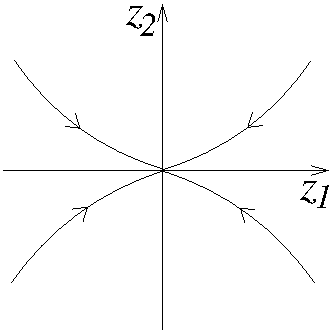
\includegraphics[width=25mm]{chap9taba1z}}&\mbox{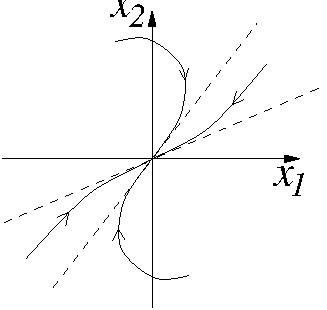
\includegraphics[width=25mm]{chap9taba1x}} &\\
\hline
\mbox{Noeud répulsif}& & & 0<\lambda_1\leq\lambda_2 \\
&\mbox{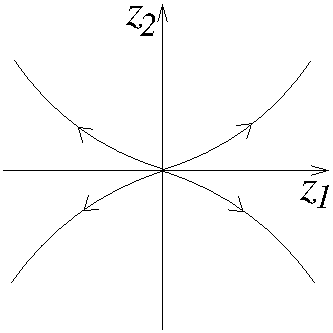
\includegraphics[width=25mm]{chap9taba2z}}& \mbox{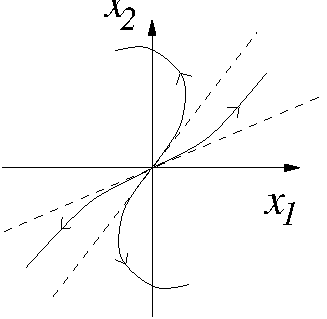
\includegraphics[width=25mm]{chap9taba2x}} &\\
\hline
\mbox{Col} & & & \lambda_1 < 0 < \lambda_2 \\
&\mbox{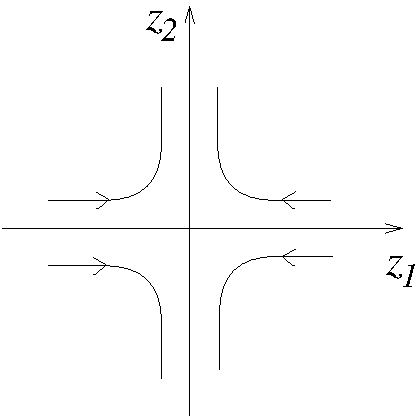
\includegraphics[width=25mm]{chap9taba3z}}& \mbox{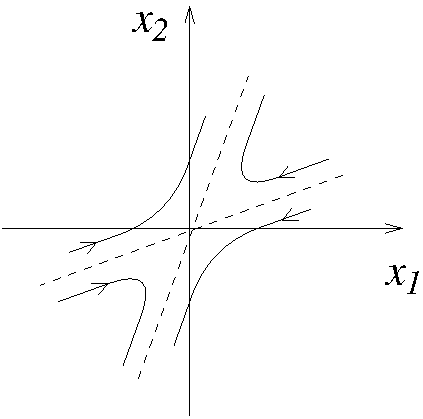
\includegraphics[width=25mm]{chap9taba3x}}&\\
\hline
\mbox{Equilibre} && &\lambda _1 = 0,  \\
\mbox{non isol{é}, attractif}&&&\lambda_2 < 0\\
&\mbox{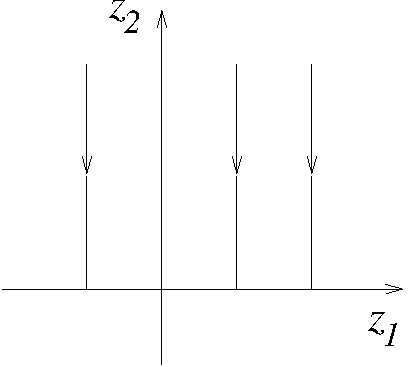
\includegraphics[width=25mm]{chap9taba4z}}&\mbox{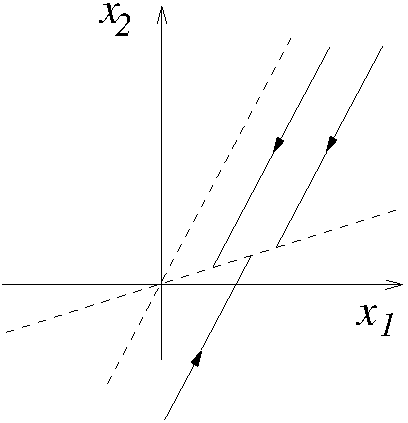
\includegraphics[width=25mm]{chap9taba4x}} &\\
\hline
\mbox{Equilibre} && &\lambda _1 = 0, \\
\mbox{non isol{é}, répulsif}&&& \lambda_2 > 0 \\
&\mbox{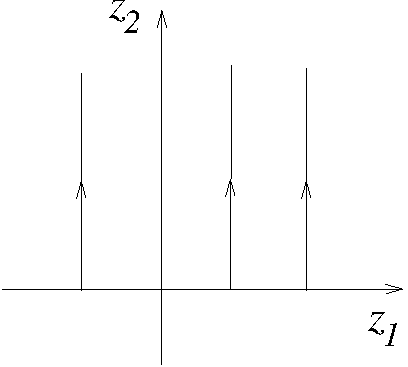
\includegraphics[width=25mm]{chap9taba5z}}& \mbox{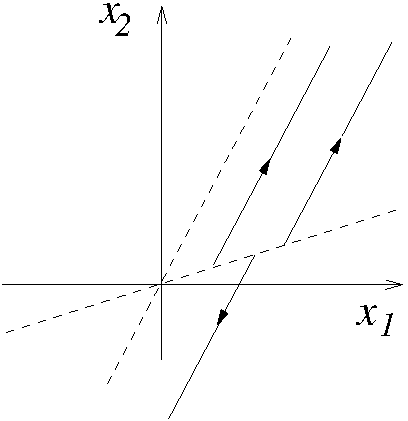
\includegraphics[width=25mm]{chap9taba5x}}&\\
\hline
\end{array}
\end{eqnarray*}
\caption{Orbites des systèmes linéaires plans~: cas\;{\em \bf a.}}
\label{tablea}
\end{table}

\begin{remarques}{\hspace{1cm}}\end{remarques}
\begin{enumerate}
\item Dans les deux premiers cas repris dans le tableau~\ref{tablea}, lorsque
$\lambda_1=\lambda_2$, les trajectoires sont rectilignes et peuvent donc
{ê}tre repr{é}sent{é}es par un faisceau de droites issu de l'origine.
\item Dans le cas ou l'une des deux valeurs propres est nulle, l'{é}quilibre
n'est pas isol{é}. Le vecteur propre correspondant {à} la valeur propre
nulle d{é}finit une droite de points d'{é}quilibre et toutes les
trajectoires sont rectilignes et convergent vers ou sont issues d'un point
de cette droite d'{é}quilibres.
\end{enumerate}
\begin{table}
\begin{eqnarray*}
\begin{array}{|c|c|c|l|}
\hline
\mbox{Type}&\mbox{Allure des}& \mbox{Allure des} &\mbox{Conditions sur}\\
\mbox{de l'{é}quilibre}&\mbox{trajectoires }(z_1,z_2)&\mbox{trajectoires }(x_1,x_2)&\mbox{les valeurs propres}\\
\hline
\begin{array}{l}
\mbox{Noeud d{é}g{é}n{é}r{é}}\\
\mbox{attractif}\end{array} & & &\begin{array}{l} \lambda = 0\\  \end{array} \mbox{(Jordan)} \\
&\mbox{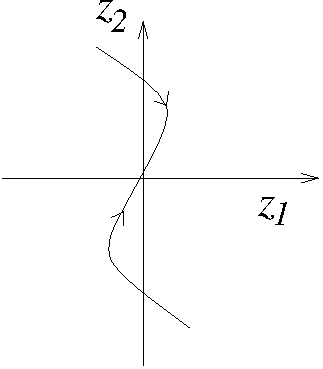
\includegraphics[width=30mm]{chap9tabB1z}}&\mbox{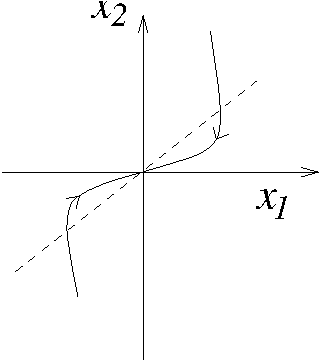
\includegraphics[width=30mm]{chap9tabB1x}} &\\
\hline
\begin{array}{l}
\mbox{Noeud d{é}g{é}n{é}r{é}}\\   
\mbox{répulsif}\end{array} & & & \begin{array}{l}\lambda >0 \\
\end{array}\mbox{(Jordan)}\\
&\mbox{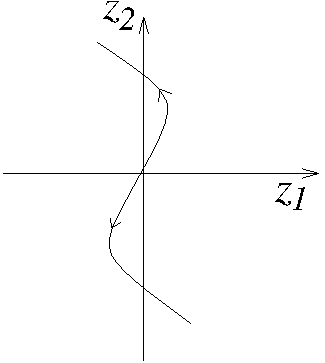
\includegraphics[width=30mm]{chap9tabB2z}}&\mbox{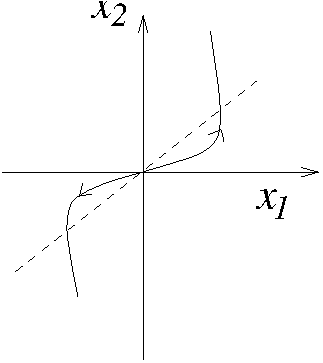
\includegraphics[width=30mm]{chap9tabB2x}} &\\
\hline
\begin{array}{l}
\mbox{Equilibre }\\   
\mbox{non-isolé}\end{array} & & & \begin{array}{l}\lambda=0\\
\end{array}\mbox{(Jordan)}\\
&\mbox{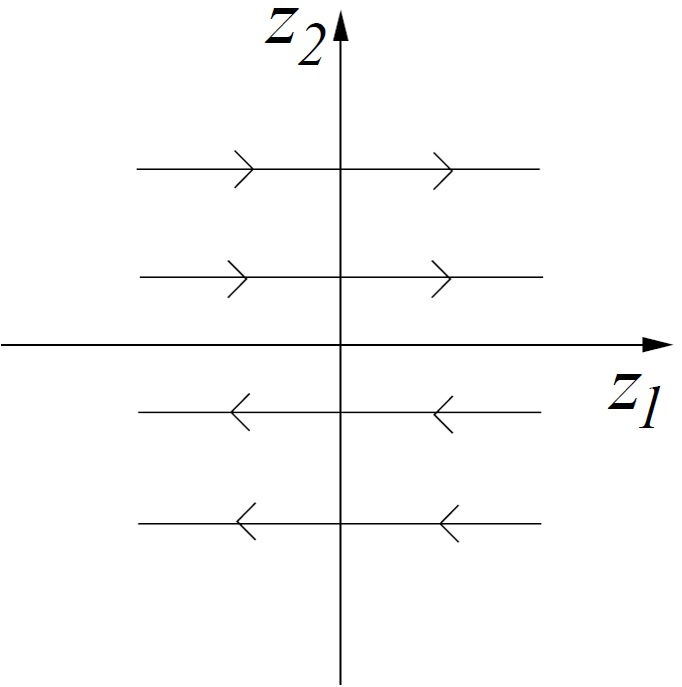
\includegraphics[width=30mm]{chap9tabB3z.jpg}}&\mbox{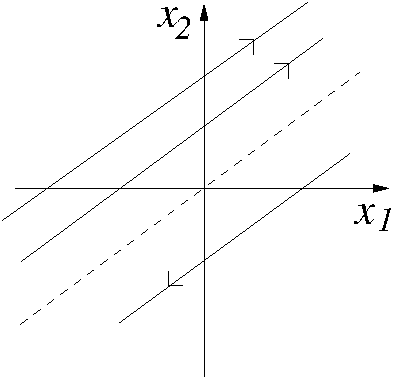
\includegraphics[width=30mm]{chap9tabB3x}} &\\
\hline
\end{array}
\end{eqnarray*}
\caption{Orbites des systèmes linéaires plans~: cas\;{\em \bf b.}}
\label{tableb}
\end{table}
%inserer ici les remarques sur le cas b)
\begin{table}
\begin{eqnarray*}
\begin{array}{|c|c|c|l|}
\hline
\mbox{Type}&\mbox{Allure des}& \mbox{Allure des} &\mbox{Conditions sur}\\
\mbox{de l'{é}quilibre}&\mbox{trajectoires }(z_1,z_2)&\mbox{trajectoires }(x_1,x_2)&\mbox{les valeurs propres}\\
\hline
\mbox{Foyer attractif} & & &\begin{array}{l}
\lambda_{1,2} = \alpha \pm \beta i\\
\alpha < 0 , \;\; \beta \neq 0 \end{array}\\
&\mbox{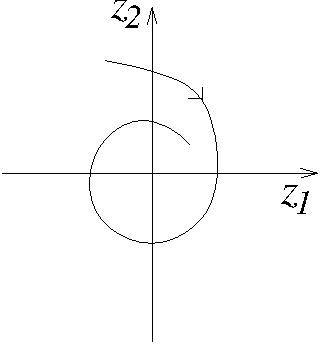
\includegraphics[width=30mm]
{chap9tabC1z}}&\mbox{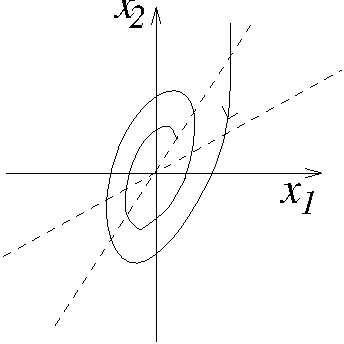
\includegraphics[width=30mm]{chap9tabC1x}} &\\
\hline
\mbox{Foyer répulsif} & & &\begin{array}{l}
\lambda_{1,2} = \alpha \pm \beta i\\
\alpha >0 , \;\; \beta \neq 0 \end{array}\\
&\mbox{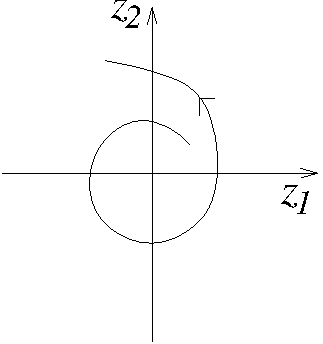
\includegraphics[width=30mm]{chap9tabC2z}}&\mbox{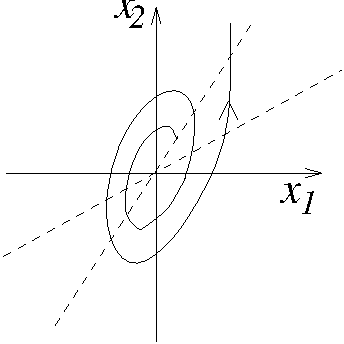
\includegraphics[width=30mm]{chap9tabC2x}} &\\
\hline
\mbox{Centre} & & &\begin{array}{l}
\lambda_{1,2} = \pm \beta i\\
 \beta \neq 0 \end{array}\\
&\mbox{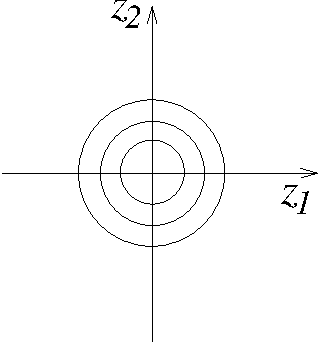
\includegraphics[width=30mm]{chap9tabC3z}}& \mbox{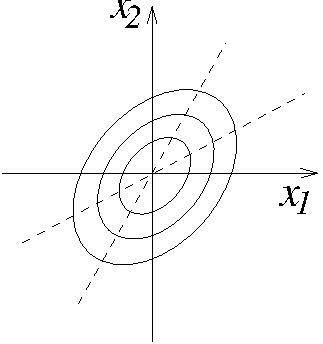
\includegraphics[width=30mm]{chap9tabC3x}}&\\
\hline
\end{array}
\end{eqnarray*}
\caption{Orbites des systèmes linéaires plans~: cas\;{\em \bf c.}}
\label{tablec}
\end{table}
\renewcommand{\arraystretch}{1.0}

\begin{definition}{\em
 Lorsque l'{é}quilibre est tel que les trajectoires con\-ver\-gent vers cet
{é}quilibre, on dira qu'il s'agit d'un {é}quilibre {\em attractif}.}\cqfd
\end{definition}

Les valeurs propres $\lambda_1$ et $\lambda_2$ de la matrice $A$ sont les racines du polyn{\^o}me  caractéristique
\eqnn
p(x)&=&x^2-(\lambda_1+\lambda_2)x +\lambda_1 \lambda_2\\
&=&x^2-\mbox{tr}(A)x+\mbox{det}A.
\eeqnn
 Observons que pour
d{é}terminer l'allure des trajectoires, il n'est pas n{é}cessaire de
calculer explicitement ces valeurs propres. La figure~\ref{fig:figlambda12}
caract{é}rise la nature de l'{é}quilibre (et d{è}s lors l'allure des
trajectoires) en fonction des deux coefficients du polyn{\^o}me
caract{é}ristique respectivement {é}gaux {à} l'oppos{é} de la somme et au
produit des valeurs propres.

\begin{figure}[htbp]
   \centering
   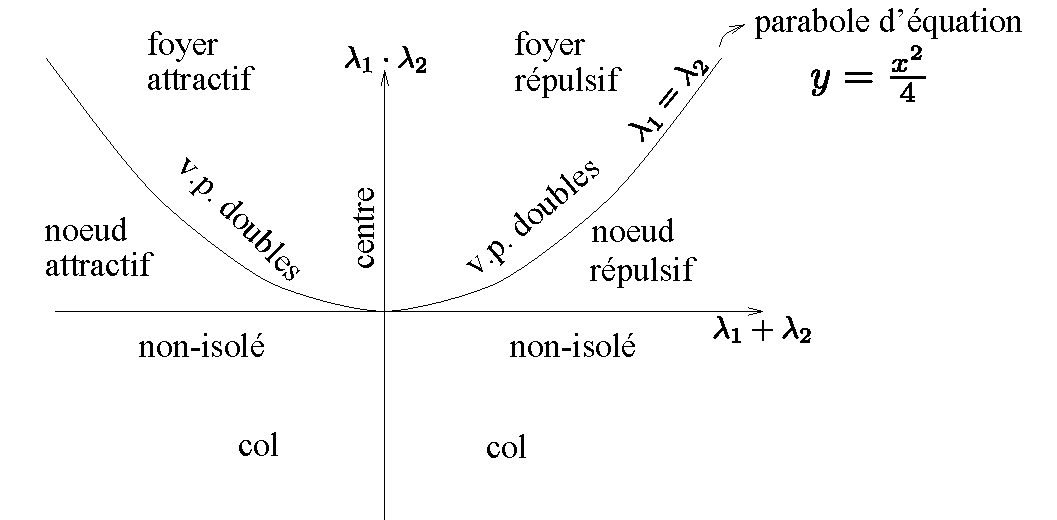
\includegraphics[width=12cm]{figlambda12} 
   \caption{
   t{é}risation des {é}quilibres en fonction de la somme et du
produit des valeurs propres}
   \label{fig:figlambda12}
\end{figure}

On peut se demander dans quelle mesure la nature des trajectoires d{é}crites
ci-dessus est sensible {à} des perturbations du syst{è}me. Pour répondre à cette question, considérons un syst{è}me lin{é}aire nominal $\dot x=
A x+Bu$ et une perturbation du syst{è}me nominal de la forme $\dot x= (A+\Delta A) x+Bu$. Si la matrice $A$ poss{è}de des valeurs
propres {\em distinctes}, on peut montrer que celles-ci d{é}pendent contin{\^u}ment
des coefficients de $A$, ce qui signifie que pour tout nombre positif
$\epsilon$, il existe un nombre positif $\delta$ tel que si chacun des
coefficients de la perturbation $\Delta A$ est plus petit que $\delta$, les
valeurs propres de la matrice perturb{é}e $A+\Delta A$ seront {à}
l'int{é}rieur de boules de rayon $\epsilon$ centr{é}es en les valeurs
propres de $A$. Donc, toute valeur propre initialement {à} l'int{é}rieur du
demi-plan de gauche ($Re(\lambda)<0$) ou du demi-plan de droite
($Re(\lambda)>0$) restera dans le m{ê}me demi-plan pour des perturbations
$\Delta A$ suffisamment petites et, qualitativement, les trajectoires du
syst{è}me perturb{é} seront semblables {à} celles du syst{è}me nominal~:
un foyer
attractif reste un foyer attractif, un noeud répulsif reste un noeud répulsif, un col reste un col,... On dit dans ce cas que de tels syst{è}mes (ou de tels {é}quilibres) sont {\em
structurellement stables}. 

Il n'en va pas de m{ê}me dans le cas d'un
{é}quilibre de type {\em centre}, auquel correspondent des trajectoires
p{é}riodiques elliptiques et des valeurs propres imaginaires pures. Dans ce
cas en effet, la moindre perturbation de la matrice $A$ peut faire en sorte
que les valeurs propres quittent l'axe imaginaire et que les trajectoires
correspondantes deviennent un foyer attractif ou répulsif. Un syst{è}me
lin{é}aire auquel correspond un {é}quilibre de type {\em centre} n'est donc
{\bf pas} structurellement stable. 

Le cas de syst{è}mes lin{é}aires ayant
une ou deux valeurs propres nulles conduit {é}galement {à} un changement
qualitatif des trajectoires sous l'effet de perturbations arbitrairement
petites. Lorsque le syst{è}me poss{è}de une valeur propre double
diff{é}rente de $0$, de petites perturbations peuvent conduire {à} des valeurs
propres r{é}elles ou complexes conjugu{é}es, mais la localisation dans l'un
ou l'autre des demi-plans ne sera pas modifi{é}e. Un noeud attractif (répulsif)
d{é}g{é}n{é}r{é} peut donc se transformer en noeud attractif (répulsif) ou en
foyer attractif (répulsif).

L'analyse pr{é}c{é}dente montre bien que c'est l'axe imaginaire qui peut
poser probl{è}me. On introduit d{è}s lors la d{é}finition suivante. 

\begin{definition} \label{hyperbolique} 
Si toutes
les valeurs propres de $A$ ont une partie r{é}elle non nulle,  le syst{è}me
$\dot x=A x$ (ou le point d'{é}quilibre)
 est dit hyperbolique. \qed 
\end{definition}

Il r{é}sulte de ce qui pr{é}c{è}de qu'un syst{è}me hyperbolique est
structurellement stable et que les trajectoires resteront qualitativement
semblables pour de petites perturbations. Dans le cas
d'une valeur propre double diff{é}rente de z{é}ro, de petites perturbations peuvent engendrer soit un foyer, soit un noeud; 
mais le caract{è}re attractif ou r{é}pulsif de l'{é}quilibre sera lui de toute fa\c{c}on 
pr{é}serv{é}.
Ces consid{é}rations vont {ê}tre
de grande importance pour l'analyse des syst{è}mes non lin{é}aires.
 

 \section{Linéarisation des systèmes non linéaires}

Les orbites illustr{é}es dans les tableaux de la section pr{é}c{é}dente ne sont pas
seulement valables au voisinage du point d'{é}quilibre (ramen{é} {à}
l'origine). On a bien caract{é}ris{é} gr{\^a}ce {à} ces tableaux l'ensemble des
orbites possibles des syst{è}mes lin{é}aires plans, quelle que soit la
condition initiale. Cette observation constitue une diff{é}rence fondamentale
entre syst{è}mes lin{é}aires et non lin{é}aires. En effet, on a vu
 au chapitre pr{é}c{é}dent que les syst{è}mes non-lin{é}aires peuvent
pr{é}senter plusieurs {é}quilibres isol{é}s distincts pour une m{ê}me
valeur de l'entr{é}e $\bar u$. Ceci implique que, contrairement au cas
des syst{è}mes lin{é}aires, le comportement des orbites au voisinage
d'un {é}quilibre gardera le plus souvent un \textit{caract{è}re local} et ne pourra
nullement
{ê}tre {é}tendu {à} l'ensemble du plan de phase. Moyennant cette
restriction, un r{é}sultat important permet cependant d'{é}tendre  aux
syst{è}mes non lin{é}aires une partie de l'analyse que nous venons de
d{é}velopper pour les syst{è}mes lin{é}aires.

Soit le syst{è}me dynamique
d{é}crit par
\eqn
\dot x_1&=&f_1(x_1,x_2, \bar u),\label{f1}\\
\dot x_2&=&f_2(x_1,x_2, \bar u).\label{f2}
\eeqn
ou, sous forme condens{é}e,
\e \label{fxu}
\dot x=f(x,\bar u),
\ee pour lequel on suppose l'existence d'un {é}quilibre $(\bar x,\bar u)$ tel que $f(\bar x,\bar u)=0$.
 On suppose en outre que la fonction $f(x,\bar u)$ est suffisamment 
 régulière dans le voisinage de cet équilibre pour y admettre un développement de Taylor convergent: 
 $$ \dot x = f(\bar{x}, \bar{u}) + \left ( \frac{\partial f(x, \bar{u})}{ \partial x}\right)_ {\bar x} {(x - \bar{x})} + \cdots . $$
L'\textit{approximation lin{é}aire} de ce syst{è}me au voisinage de l'{é}quilibre 
$(\bar x,\bar u)$, obtenue en n{é}gligeant les termes
d'ordre sup{é}rieur ou {é}gal {à} 2 dans le
d{é}veloppement de Taylor de $f(x,\bar u)$ autour de $(\bar x,\bar u)$,
est donn{é}e par
\e \label{approxli}
\dot {\tilde x} = \left ( {\frac{{\textstyle \partial f(x, \bar u)}}{{\textstyle \partial x}}} \right )_{\bar x} \tilde x 
\ee
o{ù} $\tilde x=x-\bar x$. Notons $A=\left (\frac{\partial f(x, \bar u)}{\partial x}\right )_{\bar x}$, la matrice Jacobienne de $f$ {à} l'{é}quilibre.  On peut alors g{é}n{é}raliser la d{é}finition~\ref{hyperbolique} comme suit~:
\begin{definition}\label{hyperbnl} {\bf{\em Equilibre hyperbolique}}

L'{é}quilibre $(\bar x,\bar u)$ du syst{è}me non lin{é}aire (\ref{fxu}) est
dit hyperbolique si toutes les valeurs propres de $A$ ont une partie
r{é}elle non nulle ($Re(\lambda_i(A))$ $ \neq 0, \forall i)$.\qed 
\end{definition}

Il doit {ê}tre clair que c'est bien {\em l'{é}quilibre} $(\bar x,\bar u)$ qui
est (ou qui n'est pas) hyperbolique, et non le syst{è}me non lin{é}aire
(\ref{fxu}). En effet, ce syst{è}me peut avoir plusieurs {é}quilibres
isol{é}s pour une m{ê}me valeur $\bar u$, certains {é}tant hyperboliques et
d'autres non.  Dans quelle mesure l'{é}tude de l'approximation lin{é}aire d'un syst{è}me non-lin{é}aire au voisinage d'un {é}quilibre permet-elle d'en d{é}duire le comportement du syst{è}me non-lin{é}aire~? Pour pr{é}ciser ce que l'on entend par comportement, nous voulons pouvoir comparer les trajectoires et introduisons d{è}s lors la d{é}finition suivante.

\begin{definition} 
Les trajectoires (ou les orbites) de deux systèmes dynamiques sont 
{\em topologiquement équivalentes} s'il existe un {\em homéomorphisme}
 (une bijection bicontinue) qui permet de passer d'une trajectoire du premier système 
 à une trajectoire du second. \qed
\end{definition} 

\begin{theoreme} {\bf{\em Hartman-Grobman, 1959}}

Si l'{é}quilibre $(\bar x,\bar u)$ est hyperbolique, alors les 
trajectoires du syst{è}me non
lin{é}aire~(\ref{fxu})
{\em dans un voisinage de l'{é}quilibre $(\bar x,\bar u)$} sont
topologiquement {é}quivalentes {à} celles  de l'approximation
lin{é}aire~(\ref{approxli}). Plus précisément, il existe un voisinage $X$ de $\bar x$, un voisinage $\tilde{X}$ de $0$ et un homéomorphisme $h: X \to \tilde{X}$ avec $h(\bar x)=0$
tel que si $t \mapsto x(t)$ est une trajectoire du système non 
lin{é}aire~(\ref{fxu}) contenue dans $X$ (pour un certain intervalle de temps), alors $t \mapsto h(x(t))$ est une trajectoire du système linéaire (\ref{approxli}). \label{Hart}\qed
\end{theoreme}

Des trajectoires topologiquement équivalentes ont la m{ê}me allure. On pourra donc parler de noeud ou de foyer attractif ou répulsif, ou encore de
col, pour les {é}quilibres de syst{è}mes non lin{é}aires, en {é}tudiant les valeurs propres de la matrice de l'approximation lin{é}aire, mais {\bf pas} de
centre.

\begin{remarques}\hspace{10mm}\end{remarques}

\begin{enumerate}
\item L'int{é}r{ê}t de ce th{é}or{è}me est {é}vident. Sa limitation
principale, {à} savoir son caract{è}re local, ne l'est pas moins. En
particulier, ce th{é}or{è}me ne fournit aucune indication sur la taille du
bassin d'attraction d'un {é}quilibre attractif.
\item Dans le cas d'un {é}quilibre non hyperbolique, ce sont les termes
d'ordre sup{é}rieur, ceux-l{à} m{ê}me qui ont
{é}t{é} n{é}glig{é}s, qui d{é}termineront localement l'allure des
trajectoires.
\item Les outils développés jusqu'ici dans ce chapitre ne sont pas propres au systèmes plans. Classification des systèmes linéaires, linéarisation, théorème de Hartman-Grobman se généralisent sans problème en toute dimension
\item Dans la linéarisation~(\ref{approxli}), on garde $u=\bar u$ constant. On pourrait également linéariser $f$ autour de $u=\bar u$ pour obtenir un linéarisé de type $\tilde{x}=A\tilde{x} + B\tilde{u}$. Tant que $\tilde{u}=u-\bar u$ reste suffisamment petit, et pour un intervalle de temps suffisamment petit, les trajectoires des systèmes non linéaire et linéarisé resteront proches, mais il n'existe pas de variante simple du théorème de Hartman-Grobman dans ce cas. 
\cqfd
\end{enumerate}



\section{Au delà des systèmes plans}

Les considérations précédentes ne sont pas propres aux systèmes plans. 

Le théorème d'Hartman-Grobman, par exemple, est vrai en toute dimension $n \geq 2$, 
et la classification des systèmes linéaires est semblable. 

Considérons une matrice réelle $A$ de dimension quelconque. 
Si toutes ses valeurs propres sont distinctes 
alors on peut la diagonaliser par blocs réels $1 \times 1$, 
qui contiennent une valeur propre réelle, 
ou $2 \times 2$, de la forme $$\begin{pmatrix}
\alpha& \beta\\
-\beta& \alpha
\end{pmatrix},$$
 qui encodent une paire de valeurs propres conjuguées $\alpha \pm \beta i$.
  Dans ce cas le système linéaire (ou linéarisé)
   peut se décrire comme produit direct\footnote{Une union de systèmes découplés} de système uni-dimensionnels 
   ou bi-dimensionnels comme vus dans ce chapitre.



Brièvement, le cas de blocs de Jordan est un peu différent et se comporte comme suit. Un bloc de Jordan réel, par exemple 

$$\begin{pmatrix}
\lambda& 1 & \\
       & \lambda & 1 \\
       &         & \lambda
\end{pmatrix}$$ 
engendrera une dynamique fort semblable au cas bidimensionnel, combinaison linéaires de $e^{\lambda t}$, $te^{\lambda t}$, $t^2e^{\lambda t}$:

\eqnn
z_1(t)&=&z_1(0)e^{\lambda t}+ t z_2(0)e^{\lambda t}+ t^2 z_3(0)e^{\lambda t},\\
z_2(t)&=&z_2(0)e^{\lambda t}+ t z_3(0)e^{\lambda t},\\
z_3(t)&=&z_3(0)e^{\lambda t}.
\eeqnn

Un bloc de Jordan complexe se combine avec son conjugué pour former un bloc qui ressemble par exemple à ceci:

\eqn
\begin{pmatrix}
\alpha & \beta & 1 & 0 \\
-\beta & \alpha&  0 & 1 \\
   &      &  \alpha & \beta\\
   &      &   -\beta & \alpha \\
\end{pmatrix}
\eeqn
Les solutions ressemblent alors à ceci:
\eqnn
z_1(t)&=&e^{\alpha t}(z_1(0)\cos \beta t+z_2(0) \sin \beta t+ t(z_3(0)\cos \beta t+z_4(0) \sin \beta t)),\\
z_2(t)&=&e^{\alpha t} (z_2(0)\cos \beta t-z_1(0) \sin \beta t+t(z_4(0)\cos \beta t-z_3(0) \sin \beta t)),\\
z_3(t)&=&e^{\alpha t}(z_3(0)\cos \beta t+z_4(0) \sin \beta t),\\
z_4(t)&=&e^{\alpha t}(z_4(0)\cos \beta t-z_3(0) \sin \beta t).
\eeqnn



Illustrons maintenant les sections précédentes par quelques exemples de systèmes non
linéaires d'ordre 2.



\subsection{ Les systèmes mécaniques à un degré de
liberté}

Les {é}quations d'{é}tat d'un syst{è}me m{é}canique {à} un degr{é} de libert{é}
 s'{é}crivent (voir chapitre 2)~:
\begin{align*}
\dot x_1&=x_2,\\
m\dot x_2&=-g(x_1) -k(x_1)-h(x_2) + u,
\end{align*}
o{ù} $x_1$ est la coordonn{é}e de position du corps en mouvement, $x_2$ est la vitesse, $m$ d{é}signe la masse ou l'inertie et $u$ repr{é}sente une force ou un couple 
ext{é}rieur appliqu{é} au syst{è}me. Les fonctions scalaires $g(x_1)$ et $k(x_1)$ 
correspondent respectivement {à} la gravit{é} et
{à} l'élasticité tandis que $h(x_2)$ (tel que $h(0)=0$) repr{é}sente le frottement
visqueux. Le frottement sec est n{é}glig{é}. Notons aussi (voir chapitre~2, section~2.7) que 
\eqnn
g(x_1)+k(x_1) = \frac{\partial E_p}{\partial x_1}
\eeqnn
o{ù} $E_p$ d{é}signe l'{é}nergie potentielle du syst{è}me. 

Les {é}quilibres de ce syst{è}me sont caract{é}ris{é}s par
\begin{align*}
\bar x_2 &= 0,\\
g(\bar x_1)+k(\bar x_1) &= \bar u.
\end{align*}
Sans perte de généralité, considérons le cas particulier où $m=1$. La matrice Jacobienne du syst{è}me {à} l'{é}quilibre $(\bar x_1, 0,\bar
u)$ s'{é}crit~: 
\eqnn
 A=\bma{cc} 0 & 1\\-\left (\frac{\partial^2E_p}{\partial x_1^2}\right
)_{\bar x_1} & -h'(0) \ema.
\eeqnn
Le polyn{\^o}me caract{é}ristique de cette matrice est
\eqnn
p(x)=x^2+h'(0)x+\left (\frac{\partial^2E_p}{\partial x_1^2}\right )_{\bar
x_1}.
\eeqnn
 Le produit et la somme des valeurs propres sont donn{é}s par
$$ \lambda_1\lambda_2=\left (\frac{\partial^2E_p}{\partial x_1^2}\right
)_{\bar x_1}, \;\;\; \lambda_1+\lambda_2=-h'(0).$$
La d{é}riv{é}e $h'(0)$ du frottement visqueux est 
par nature non-n{é}gative~: $\lambda_1+\lambda_2 =-h'(0) \leq 0$.




Les {é}quilibres du syst{è}me sont hyperboliques si
 \eqnn 
h'(0) >0 &\mbox{et }&  \left (\frac{\partial^2E_p}{\partial x_1^2}\right
)_{\bar x_1} \neq 0,\\
 \mbox{ou si }  h'(0) =0 &\mbox{et }& \left (\frac{\partial^2E_p}{\partial x_1^2}\right
)_{\bar x_1} < 0.
\eeqnn
On observe donc que les {é}quilibres ne sont {\em pas} hyperboliques si l'{é}nergie potentielle $E_p(x_1)$ est une fonction affine de la position $x_1$, ou plus g{é}n{é}ralement si l'{é}quilibre correspond {à} un point d'inflexion de $E_p(x_1)$. C'est {é}galement le cas lorsque  $h'(0)=0$ et $\left (\frac{\partial^2E_p}{\partial
x_1^2}\right )_{\bar x_1} \geq 0$.

Les {é}quilibres hyperboliques d'un syst{è}me m{é}canique {à} un degr{é} 
de libert{é} peuvent alors {ê}tre compl{è}tement caract{é}ris{é}s 
comme indiqu{é} au tableau~\ref{tab:tabsysmec} (voir aussi la figure~\ref{fig:eqsysmec}).
\begin{figure}[t] 
   \centering
   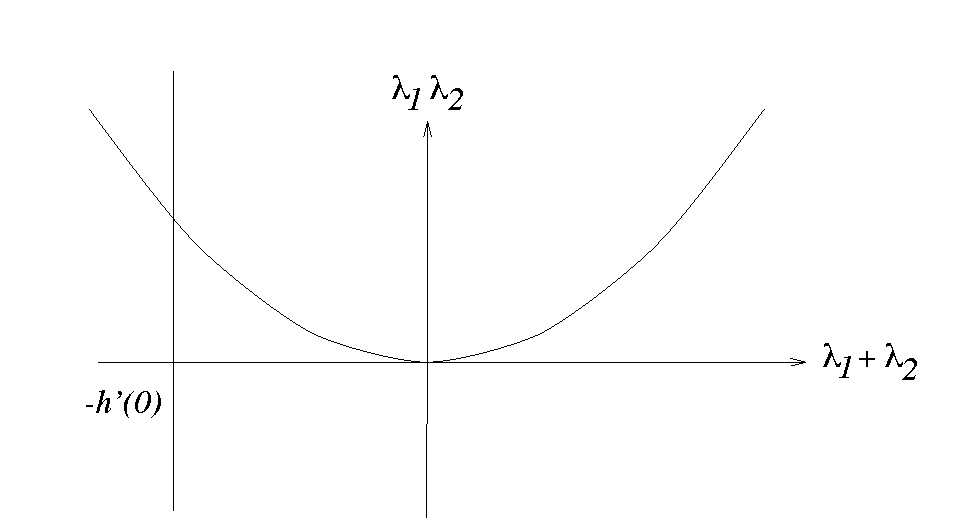
\includegraphics[height=4cm]{eqsysmec} 
   \caption{Lieu des valeurs propres des équilibres d'un syst{è}me m{é}canique {à} un degr{é} de libert{é}}
   \label{fig:eqsysmec}
\end{figure}
\begin{table}
\hspace*{5mm}
%\renewcommand{\arraystretch}{1.2}
\begin{tabular}{|c|c|}
\hline
Caract{é}risation&Nature des {é}quilibres hyperboliques\\ \hline
{}&{}\\
$0< [h'(0)]^2 <4 \left (\frts{\partial^2E_p}{\partial x_1^2}\right
)_{\bar x_1}$&foyer stable \\
{}&{}\\ \hline
{}&{}\\
$0<4 \left (\frts{\partial^2E_p}{\partial x_1^2}\right
)_{\bar x_1}\leq [h'(0)]^2$&noeud stable \\
{}&{}\\
 \hline
 {}&{}\\
$\left (\frts{\partial^2E_p}{\partial x_1^2}\right
)_{\bar x_1} <0$&col \\ 
{}&{}\\
\hline
\end{tabular}
\caption{Equilibres hyperboliques des syst{è}mes m{é}caniques à un degré
de liberté}
\label{tab:tabsysmec}
\end{table}
On observe en particulier qu'un {é}quilibre hyperbolique ne peut jamais {ê}tre un noeud ou un foyer répulsif.

\subsection{Les circuits électriques RLC}

Les circuits {é}lectriques simples qui ne contiennent qu'une inductance et 
une capacit{é} sont g{é}n{é}ralement d{é}nomm{é}s {\em circuits 
RLC} dans la litt{é}rature. Dans les ouvrages de r{é}f{é}rence en 
g{é}nie {é}lectrique ou en th{é}orie des circuits, ils font l'objet 
d'une {é}tude approfondie car ils constituent la configuration de base de
 nombreux dispositifs pratiques (filtres, oscillateurs,...).

Le circuit {\em RLC s{é}rie} repr{é}sent{é} {à} la figure~\ref{fig:RLCs}
est un exemple typique.
\begin{figure}[htbp] 
   \centering
   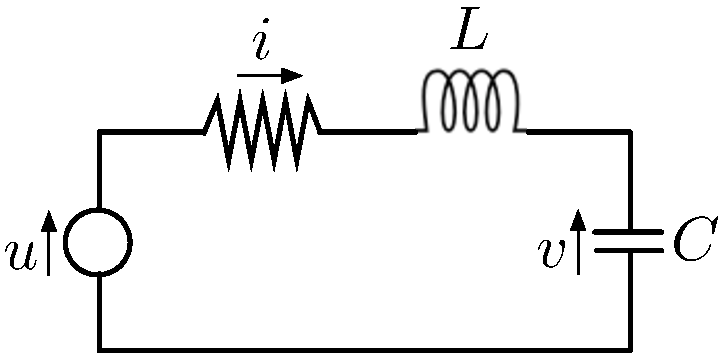
\includegraphics[height=2.5cm]{RLCs} 
   \caption{Circuit RLC s{é}rie}
   \label{fig:RLCs}
\end{figure}
En application des principes {é}tudi{é}s au chapitre~3, le 
comportement dynamique de ce circuit est d{é}crit par un mod{è}le 
d'{é}tat de dimension 2~:
\eqnn
L \dot x_1&=&-r(x_1)-x_2 +u\\
C \dot x_2&=&x_1
\eeqnn
o{ù} $x_1=i$ est le courant dans l'inductance linéaire $L$, $x_2=v$ est 
la tension aux bornes de la capacit{é} linéaire $C$ et $r(x_1)$ est la 
caract{é}ristique tension-courant ({é}ventuellement non lin{é}aire)
de la r{é}sistance.
\begin{figure}[t] 
   \centering
   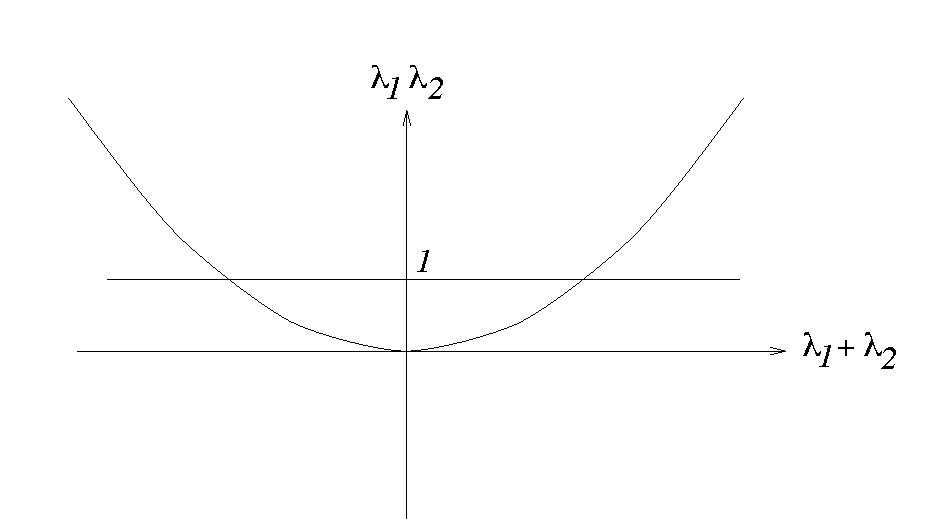
\includegraphics[height=4cm]{figrlc} 
   \caption{Lieu des valeurs propres des {é}quilibres d'un circuit RLC}
   \label{fig:figrlc}
\end{figure}

Les {é}quilibres de ce syst{è}me sont caract{é}ris{é}s par 
les {é}quations~:
\begin{align*}
\bar x_2 +r(0) &= \bar u,\\
\bar x_1 &= 0.
\end{align*}
Sans perte de généralité, considérons le cas particulier $L=1$ et $C=1$. La matrice Jacobienne du syst{è}me {à} l'{é}quilibre $(0,\bar x_2,\bar u)$ s'{é}crit~:
$$A=\bma{cc} -r'(0) & -1\\1&0\ema .$$
Le polyn{\^o}me caract{é}ristique de cette matrice est~:
\eqnn
p(x)&=&\lambda^2+r'(0) \lambda +1\\
\mbox{o{ù} }\;\; r'(0)&\triangleq&(\partial r/\partial x_1)_{x_1=0}.
\eeqnn
Le produit et la somme des valeurs propres sont donn{é}s par
$$ \lambda_1\lambda_2=1,  \;\;\; \lambda_1+\lambda_2=-r'(0).$$
Les {é}quilibres du syst{è}me sont donc hyperboliques si $r'(0)\neq 0$, 
c.{à}.d. si la d{é}riv{é}e de la caract{é}ristique de la r{é}sistance n'est pas 
nulle {à} l'origine. On observe que c'est notamment le cas pour une 
r{é}sistance lin{é}aire.

Les {é}quilibres hyperboliques d'un circuit RLC s{é}rie sont alors compl{è}tement
caract{é}ris{é}s comme indiqu{é} sur le tableau \ref{tabrlc} 
(voir aussi la figure~\ref{fig:figrlc}).
\begin{table}
\centering
\renewcommand{\arraystretch}{3.0}
\begin{tabular}{|c|c|}
\hline
&Nature des {é}quilibres hyperboliques\\ \hline
$r^{'}(0) \geq 2$&noeud attractif \\ \hline
$0 < r^{'}(0) < 2$&foyer attractif \\ \hline
$-2 < r^{'}(0) < 0$&foyer répulsif \\ \hline
$r^{'}(0) \leq -2 $& noeud répulsif\\
\hline
\end{tabular}
\caption{Equilibres hyperboliques d'un circuit RLC}\label{tabrlc}
\end{table}
On remarque en particulier qu'un {é}quilibre hyperbolique d'un circuit RLC s{é}rie ne peut jamais {ê}tre un col.

\subsection{Les systèmes à deux compartiments}

Consid{é}rons les syst{è}mes {à} deux compartiments dont le graphe est repr{é}sent{é} {à} la
figure~\ref{fig:deuxcomp}.
\begin{figure}[htbp] 
   \centering
   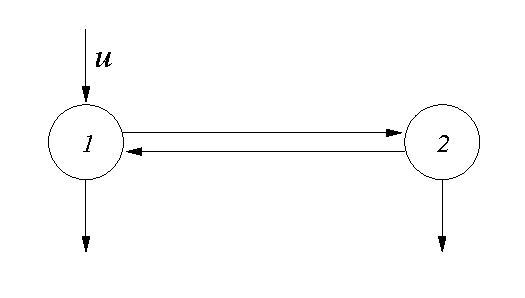
\includegraphics[height=4cm]{deuxcomp} 
   \caption{Système à deux compartiments}
   \label{fig:deuxcomp}
\end{figure}
Le signal d'entr{é}e $u$ est le d{é}bit d'alimentation du premier compartiment.  Nous
supposons que les flux {é}chang{é}s entre les compartiments satisfont les conditions
$C1 - C4$ de mod{é}lisation du chapitre 4 (Section 4.3).  La dynamique du syst{è}me
est alors d{é}crite par un mod{è}le d'{é}tat de dimension 2 de la forme g{é}n{é}rale
suivante :
\eqnn
\dot x_1 &=& -q_{12} (x_1, x_2) + q_{21} (x_2,x_1) - q_{10} (x_1) + u\\
\dot x_2 &=& q_{12}(x_1,x_2)-q_{21} (x_2,x_1) - q_{20} (x_2)
\eeqnn
Les fonctions $q_{ij}$ satisfont les conditions suivantes
sur l'orthant positif :
\e
q_{ij}(0, x_j) = 0 \;\;\; \frac{\partial q_{ij}}{\partial
x_{i}} \geq 0 \;\; \frac{\partial q_{ij}}{\partial
x_{j}} \leq 0 \label{orthpositif}
\ee
Sous ces conditions, le
syst{è}me poss{è}de une infinit{é} d'{é}quilibres isol{é}s positifs
$(\bar x_1, \bar x_2, \bar u)$.  La matrice Jacobienne
autour de l'un de ces {é}quilibres s'{é}crit :
$$
A = \bma{cc} -(a+c) &  b\\a & -(b+d) 
\ema
$$
avec les notations simplifi{é}es suivantes (toutes les
d{é}riv{é}es partielles sont {é}valu{é}es {à} l'{é}tat d'{é}quilibre ) :
\eqnn
a &\triangleq & \frac{\partial q_{12}}{\partial x_1} - \frac{\partial
q_{21}}{\partial x_1} \hspace*{15mm}c \triangleq \frac{\partial q_{10}}{\partial x_1}\\
b &\triangleq & \frac{\partial q_{21}}{\partial x_2} - \frac{\partial
q_{12}}{\partial x_2} \hspace*{15mm} d \triangleq \frac{\partial q_{20}}{\partial x_2}
\eeqnn
Sous les conditions (\ref{orthpositif}), on observe imm{é}diatement que
$a,b,c,d, \geq~0$.  Le polyn{\^o}me caract{é}ristique de la matrice Jacobienne s'{é}crit :
$$
p(x) = x^2 + (a+b+c+d)x + (ad+bc+cd)
$$
Le produit et la somme des valeurs propres sont donc donn{é}s par :
$$
\lambda_1 \lambda_2 = ad+bc+cd \;\;\;\; \lambda_1 + \lambda_2 = -(a+b+c+d)
$$
Les {é}quilibres du syst{è}me sont donc hyperboliques si les in{é}galit{é}s suivantes
sont satisfaites :
$$
a+b+c+d > 0 \;\;\mbox{ et }\;\; ad+bc+cd > 0
$$
On d{é}montre ais{é}ment que, sous ces conditions, l'in{é}galit{é} suivante est aussi
satisfaite :
$$
0<4 (ad+bc+cd) \leq (a+b+c+d)^2
$$
On en d{é}duit que les {é}quilibres hyperboliques d'un syst{è}me {à} deux
compartiments ne peuvent {ê}tre que des noeuds attractifs (voir
figure~\ref{fig:eq2comp}).
\begin{figure}[htbp] 
   \centering
   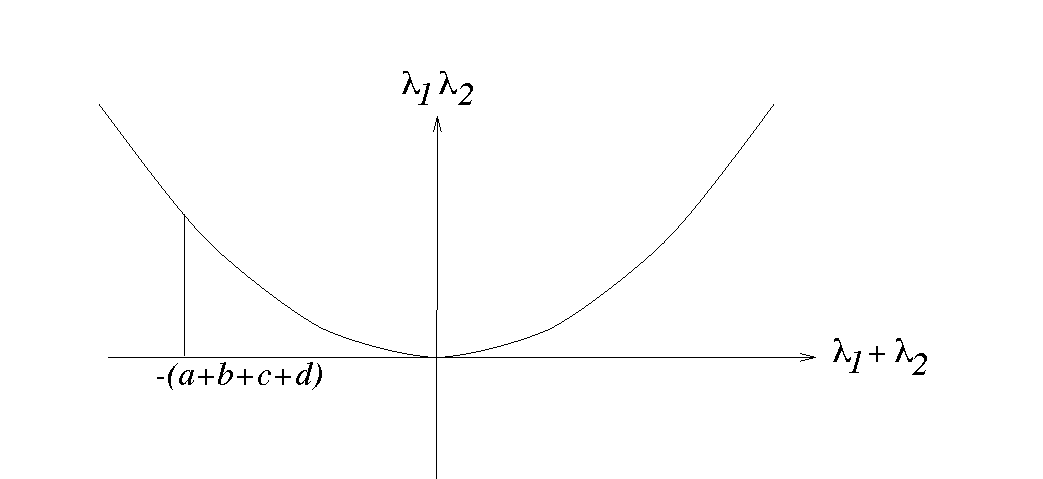
\includegraphics[height=4cm]{eq2comp} 
   \caption{Lieu des valeurs propres des {é}quilibres d'un syst{è}me {à} 
deux compartiments}
   \label{fig:eq2comp}
\end{figure}

\subsection{Les systèmes réactionnels à deux espèces}

Les syst{è}mes r{é}actionnels les plus simples font intervenir deux esp{è}ces. 
C'est le cas par exemple d'une r{é}action irr{é}versible convertissant un r{é}actif
$X_1$ en un produit $X_2$ :
$$
X_1 \longrightarrow X_2
$$
Supposons que cette r{é}action se d{é}roule dans un r{é}acteur continu parfaitement
m{é}lang{é} {à} volume constant.  Le r{é}acteur est aliment{é} avec l'esp{è}ce
 $X_1$, {à}
d{é}bit volum{é}trique constant strictement positif.  Comme nous l'avons vu au
chapitre 5, le mod{è}le d'état du r{é}acteur peut s'{é}crire comme suit :
\eqnn
\dot x_1 &=& -r(x_1,x_2) + d(u-x_1)\\
\dot x_2 &=& r(x_1,x_2) - dx_2
\eeqnn
o{ù}  $x_1$ et $x_2$ représentent les concentrations des esp{è}ces $X_1$ et $X_2$ dans le
milieu r{é}actionnel, $d$ est le taux de dilution et $u$ est la concentration du
r{é}actif $X_1$ dans l'alimentation.  La cin{é}tique de r{é}action $r(x_1,x_2)$ est
suppos{é}e {ê}tre une fonction des concentrations des deux esp{è}ces.
\begin{figure}[t] 
   \centering
   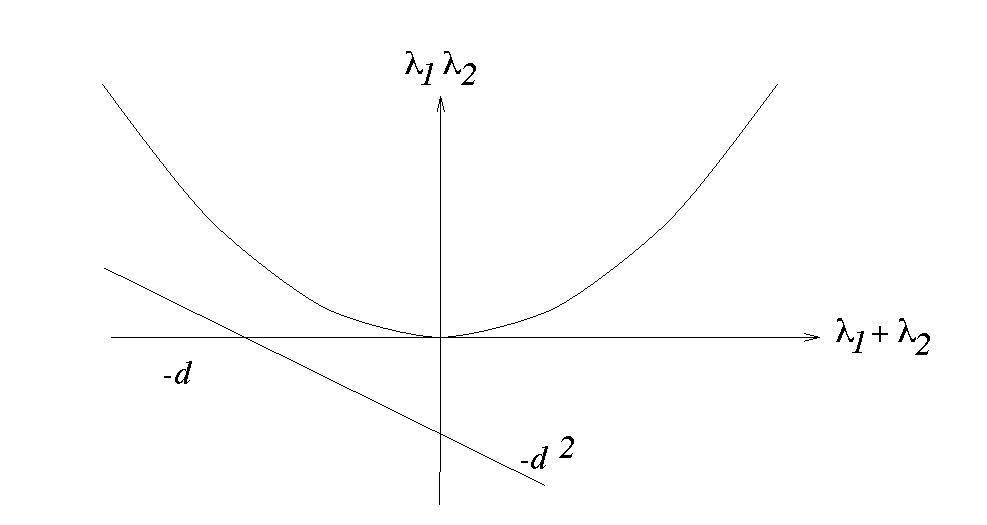
\includegraphics[height=4cm]{fig2esp} 
   \caption{Lieu des valeurs propres des {é}quilibres d'un syst{è}me
 r{é}actionnel {à} deux esp{è}ces}
   \label{fig:fig2esp}
\end{figure}

Les {é}quilibres du syst{è}me sont donc caract{é}ris{é}s par les {é}quations  :
$$
d\bar x_2 = d(\bar u-\bar x_1) = r(\bar x_1, \bar x_2)
$$
Ces {é}quations impliquent {à} l'{é}quilibre que $\bar x_1 + \bar x_2 = \bar u$,
c'est {à} dire que la somme des concentrations des esp{è}ces $X_1$ et $X_2$ dans le
r{é}acteur est {é}gale {à} la concentration du r{é}actif $X_1$ dans l'alimentation. 
Cette observation est {é}videmment en accord avec le principe de conservation de
la masse.

La matrice Jacobienne autour de l'{é}quilibre s'{é}crit :
$$
A = \bma{cc}
-a-d & -b \\a & b-d
\ema
$$
avec les notations simplifi{é}es suivantes :
$$
a  \triangleq \left( \frac{\partial r(x_1,x_2)}{\partial x_1} \right )_{\bar
x_1, \bar x_2} \hspace*{15mm} b \triangleq \left( \frac{\partial r(x_1,x_2)}{\partial x_2} \right )_{\bar
x_1, \bar x_2} 
$$
Le polyn{\^o}me caract{é}ristique de la matrice Jacobienne s'{é}crit :
$$
p(x) = x^2 + (a-b +2d) x + (a-b) d +d^2
$$
Le produit et la somme des valeurs propres sont donc donn{é}s par :
$$
\lambda_1 \lambda_2 = (a-b)d+d^2 \;\;\;\; \lambda_1 + \lambda_2 = -(a-b+2d)
$$
Etant donn{é} que le taux de dilution $d$ est une quantit{é} strictement positive,
on peut v{é}rifier apr{è}s quelques calculs que les {é}quilibres du syst{è}me sont
hyperboliques si $(a-b) \neq -d$. On observe que 
\begin{itemize}
\item si $\lambda_1 + \lambda_2 = -[(a-b)+2d]>0$, alors n{é}cessairement
$\lambda_1 \lambda_2 = d[(a-b)+d]<0$ et donc l'{é}quilibre est un col.
\item Si $\lambda_1 + \lambda_2 = -[(a-b)+2d]\leq 0$, alors l'{é}quilibre est un col
si $-2d\leq(a-b)<-d$, et un noeud attractif si $(a-b)>-d$.  Par contre,
l'{é}quilibre ne peut pas {ê}tre un foyer, car il est impossible d'avoir
$\lambda_1 \lambda_2 \geq \frac{1}{4} (\lambda_1 + \lambda_2)^2$.
\end{itemize}
Cette analyse est r{é}sum{é}e dans 
le tableau~\ref{tab2esp} et la figure~\ref{fig:fig2esp}.

\begin{table}
\hspace*{10mm}
\renewcommand{\arraystretch}{3.0}
\begin{tabular}{|c|c|}
\hline
&Nature des {é}quilibres hyperboliques\\ \hline
$(a-b)<-d$&col \\ \hline
$(a-b)>-d$&noeud attractif \\ \hline
\end{tabular}
\caption{Equilibres hyperboliques d'un syst{è}me r{é}actionnel {à} deux esp{è}ces}
\label{tab2esp}
\end{table}

\section{Trajectoires p{é}riodiques et cycles limites}

A partir des tableaux de la section~8.2, on peut tirer les
observations suivantes.
\begin{enumerate}
\item Pour un syst{è}me lin{é}aire de dimension deux, les équilibres {\em
attractifs} sont soit un noeud  soit un foyer, soit enfin une droite d'{é}quilibres non isol{é}s. Dans
chacun de ces cas, le bassin d'attraction est le plan de phase tout entier.
\item Lorsque l'{é}quilibre est r{é}pulsif, les trajectoires du
syst{è}me divergent lorsque le temps $t$ tend vers l'infini.
\item Lorsque l'{é}quilibre d'un syst{è}me lin{é}aire est un centre, toutes
les trajectoires du syst{è}me sont p{é}riodiques et le rayon des 
trajectoires d{é}pend des conditions initiales.
Un syst{è}me lin{é}aire pr{é}sentant des trajectoires p{é}riodiques
est structurellement instable, et donc la moindre perturbation du syst{è}me
peut faire dispara\^ \i tre ces trajectoires p{é}riodiques. 
\end{enumerate}

Aucune de ces observations n'est v{é}rifi{é}e g{é}n{é}riquement dans le cas de
syst{è}mes non lin{é}aires. En effet, les deux premi{è}res concernent un
comportement {\em global} des trajectoires, et nous avons vu que ce n'est
que localement, dans le voisinage d'un {é}quilibre hyperbolique, que les
trajectoires d'un syst{è}me non lin{é}aire se comportent comme celles de
l'approximation lin{é}aire de ce syst{è}me. L'objet de cette section est de
montrer que pour des syst{è}mes non lin{é}aires, il existe d'autres
ensembles attractifs et notamment des trajectoires p{é}riodiques.
 On montrera en outre que ces ensembles
attractifs sont
structurellement stables. Ceci est une propri{é}t{é} tr{è}s intéressante des 
syst{è}mes non lin{é}aires qui est utilis{é}e pour la conception de circuits oscillateurs.
\begin{exemple} {\bf  \em Circuit RLC {à} diode tunnel} 

\begin{figure}[htbp] 
   \centering
   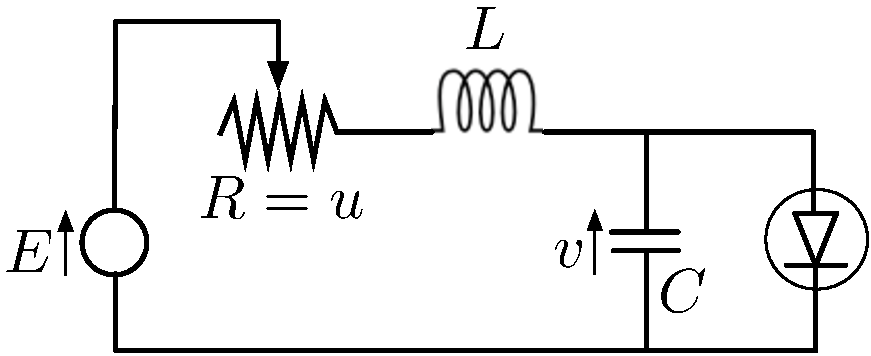
\includegraphics[height=25mm]{osc} 
   \caption{Oscillateur {à} diode tunnel}
   \label{fig:osc}
\end{figure}

La figure~\ref{fig:osc} repr{é}sente un oscillateur {à} diode tunnel. C'est  un circuit
{é}lectrique RLC comprenant des dip{\^o}les lin{é}aires (une source de tension constante
$E$, une r{é}sistance linéaire $R$ variable, une inductance linéaire
$L= 1H$, une capacit{é} linéaire $C=1F$) ainsi qu'une r{é}sistance non lin{é}aire (diode tunnel)
dont la caract{é}ristique courant-tension $i=h(v)=2v^3-6v^2+5v$ a l'allure de la courbe
repr{é}sent{é}e {à} la figure~\ref{fig:diode}. L'entr{é}e $u$ de ce syst{è}me est la
r{é}sistance variable $R$.
\begin{figure}[htbp] 
   \centering
   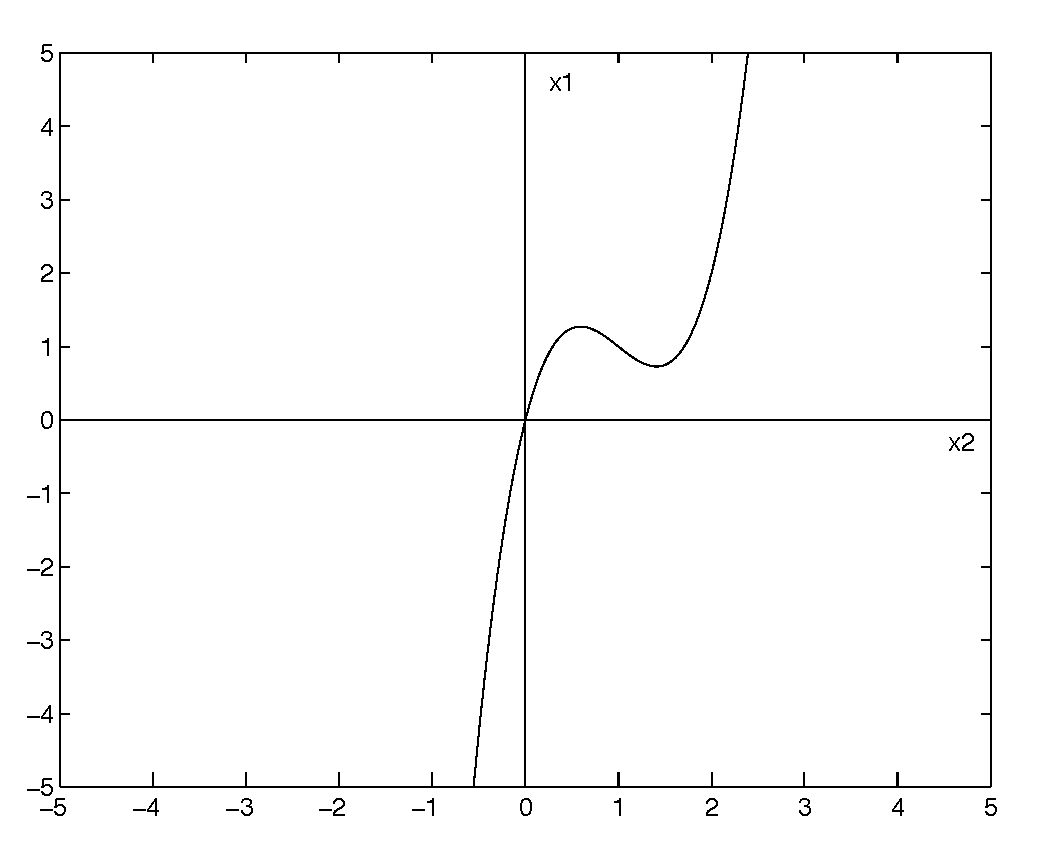
\includegraphics[width=10cm]{caradio} 
   \caption{Caract{é}ristique courant-tension de la diode tunnel}
   \label{fig:caradio}
\end{figure}
Comme nous l'avons vu au chapitre~3, les  variables d'{é}tat du syst{è}me sont le courant
$x_1=i$  dans l'inductance et  la tension 
$x_2=v$ aux bornes de la capacit{é}.  On obtient les
{é}quations d'{é}tat suivantes~:
\eqnn
\dot x_1&=&-u x_1-x_2 +E\\
\dot x_2&=&x_1-h(x_2),
\eeqnn
et les {é}quilibres possibles sont caract{é}ris{é}s par
\eqnn
\bar x_1&=&\frac{E -\bar x_2}{\bar u}\\
\bar x_1&=&h(\bar x_2).
\eeqnn

En repr{é}sentant dans le plan de phase les graphes des courbes $
\bar x_1=(E -\bar x_2)/\bar u$ et $\bar x_1=h(\bar x_2)$, on constate que, pour une
diode de caract{é}ristique donn{é}e, deux configurations sont possibles selon les valeurs
respectives de
$\bar u$ et $E$. Si la pente de la droite ($-1/\bar u$) est
suffisamment raide, il n'y aura qu'un seul point d'{é}quilibre
(figure~\ref{fig:eqdiode}.a).  Par contre, si cette
pente est inf{é}rieure {à} celle de la tangente au point d'inflexion de la courbe, il y
aura un, deux ou trois {é}quilibres possibles suivant la valeur de $E$
(figure~\ref{fig:eqdiode}.b).
\begin{figure}[htbp] 
   \centering
   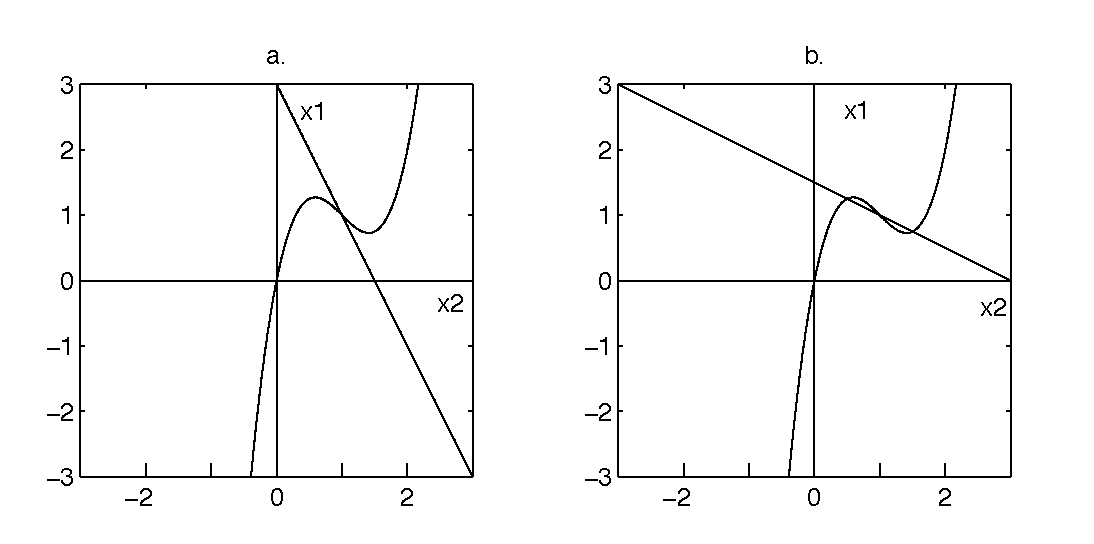
\includegraphics[width=10cm]{eqdiode} 
   \caption{Configurations d'{é}quilibres pour le circuit avec diode tunnel}
   \label{fig:eqdiode}
\end{figure}

On peut {à} nouveau {é}tudier l'allure des trajectoires au voisinage des
{é}quilibres en calculant les valeurs propres de la matrice Jacobienne du
syst{è}me~:
$$A=\bma{cc} -\bar u & -1\\1&-h'(\bar x_2)\ema .$$
Le produit et la somme des valeurs propres sont donn{é}s par
$$ \lambda_1\lambda_2=\bar u h'(\bar x_2) +1,  \;\;\; \lambda_1+\lambda_2=-(\bar u+
h'(\bar x_2)),$$
et on observe que le signe des valeurs propres ne d{é}pend pas de $E$
mais seulement des pentes respectives des deux graphes de l'une ou l'autre
des figures~\ref{fig:eqdiode}.

Examinons en d{é}tail les  {é}quilibres~: 
\begin{itemize}
\item[{\bf a.}] Pour la figure~\ref{fig:eqdiode}.a, il n'y a qu'un seul {é}quilibre. Si celui-ci
 se
trouve {à} gauche du maximum local de la courbe $h(x_2)$ ou {à} droite du minimum local de
celle-ci, le produit des valeurs propres est positif, la somme est n{é}gative et
l'{é}quilibre correspondant est donc un noeud ou un foyer attractif. 
\item[{\bf b.} ] Toujours pour la premi{è}re figure, si l'{é}quilibre se trouve entre le maximum
et le minimum locaux, on a $-1/\bar u < h'(\bar x_2)<0$ et le produit des valeurs propres
est donc toujours positif. Quant {à} la somme, elle sera n{é}gative et l'{é}quilibre
correspondant d{è}s lors attractif si $|h'(\bar x_2)|<\bar u$ (ce qui correspond {à} une
valeur de
$\bar u$ importante, c.{à}.d. une résistance fortement dissipative qui assure la
stabilit{é} du circuit). Par contre, si $|h'(\bar x_2)|>\bar u$, la somme des valeurs
propres est positive et l'{é}quilibre correspondant est répulsif.
\item[{\bf c.}] Pour la figure~\ref{fig:eqdiode}.b,  les {é}quilibres {à} gauche du maximum local de
$h(x_2)$ et {à} droite du minimum local sont tels que le produit des valeurs propres est
positif et la somme des valeurs propres est n{é}gative. L'{é}quilibre correspondant est
donc un noeud ou un foyer attractif.
\item[{\bf d.}]  Quant {à} l'{é}quilibre {é}ventuel compris entre maximum et minimum, il v{é}rifie $h'(\bar x_2) < -1/\bar u < 0$. Le produit des
valeurs propres est n{é}gatif et l'{é}quilibre correspondant est un col.
\end{itemize}

Comme on peut le constater, l'{é}quilibre est répulsif dans diff{é}rents cas. On peut 
alors s'interroger sur ce que deviennent les trajectoires qui s'{é}loignent de ce point
d'{é}quilibre. Consid{é}rons les valeurs num{é}riques
particuli{è}res suivantes~:
\eqnn
\bar u&=&0.5,\\
E&=& 1.5,\\
h(v)&=&2v^3-6v^2+5v.
\eeqnn
On peut v{é}rifier que pour ces valeurs
particuli{è}res, $(\bar x_1, \bar x_2, \bar u)= (1,1,0.5)$ est le seul
{é}quilibre du syst{è}me, et qu'il s'agit d'un {é}quilibre r{é}pulsif (cas {\bf b.}
ci-dessus). 

En simulant le syst{è}me de deux {é}quations
diff{é}rentielles pour diff{é}rentes conditions initiales, on obtient les orbites
illustr{é}es  
{à} la figure~\ref{fig:diode}. Il apparaît clairement que toutes
les orbites calcul{é}es (on peut penser que les autres se comporteraient de la m{ê}me
mani{è}re) s'enroulent autour d'une orbite p{é}riodique. Ce syst{è}me ne
poss{è}de donc pas d'{é}quilibre attractif, mais il existe une {\em
orbite ferm{é}e} qui est attractive. C'est ce qu'on appelle un
cycle limite.
\begin{figure}[htbp] 
   \centering
   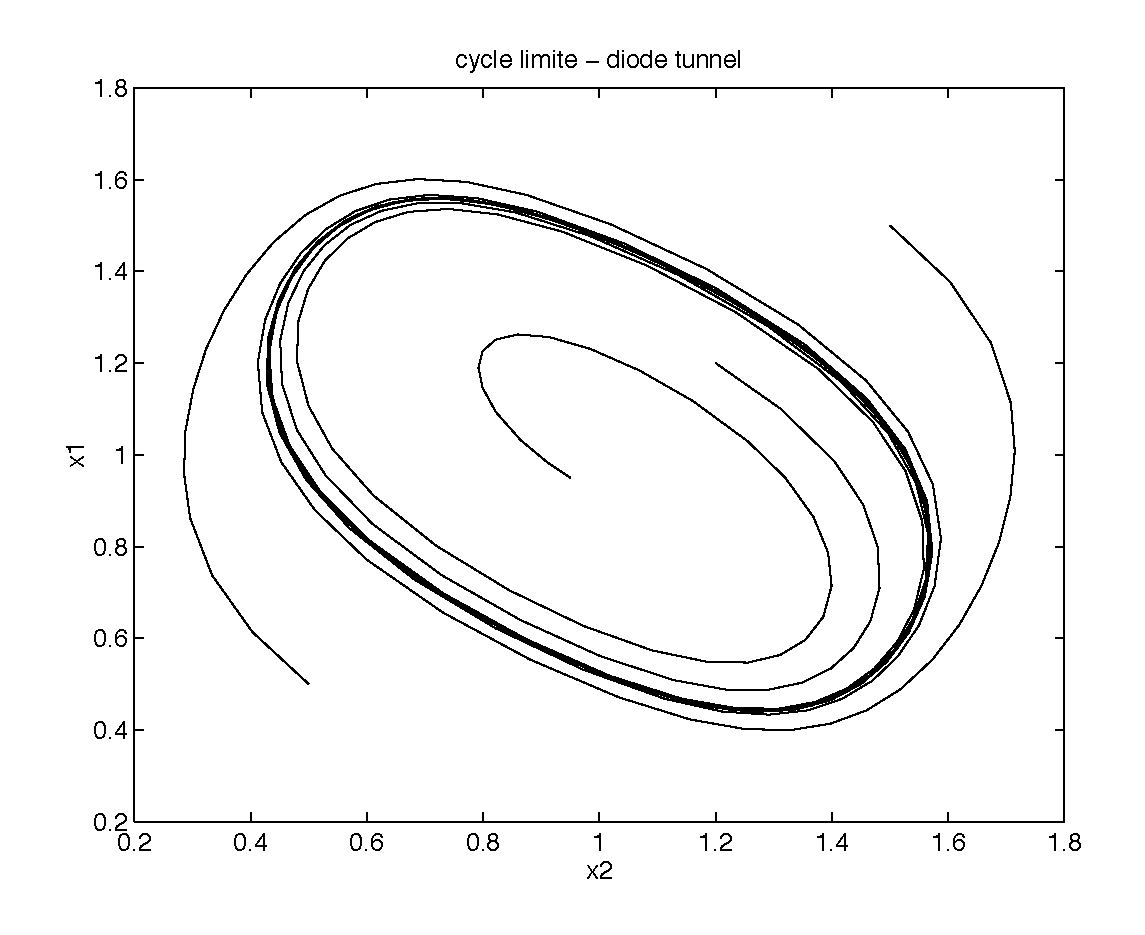
\includegraphics[width=10cm]{diode} 
   \caption{Cycle limite pour le circuit {à} diode tunnel}
   \label{fig:diode}
\end{figure}
La figure~\ref{fig:simudiodet} illustre les trajectoires ({é}tat en fonction du temps) et 
montre bien qu'elles convergent (rapidement) vers des trajectoires p{é}riodiques dont la
p{é}riode et l'amplitude ne d{é}pendent pas des conditions initiales.
\begin{figure}[htbp] %  figure placement: here, top, bottom, or page
   \centering
   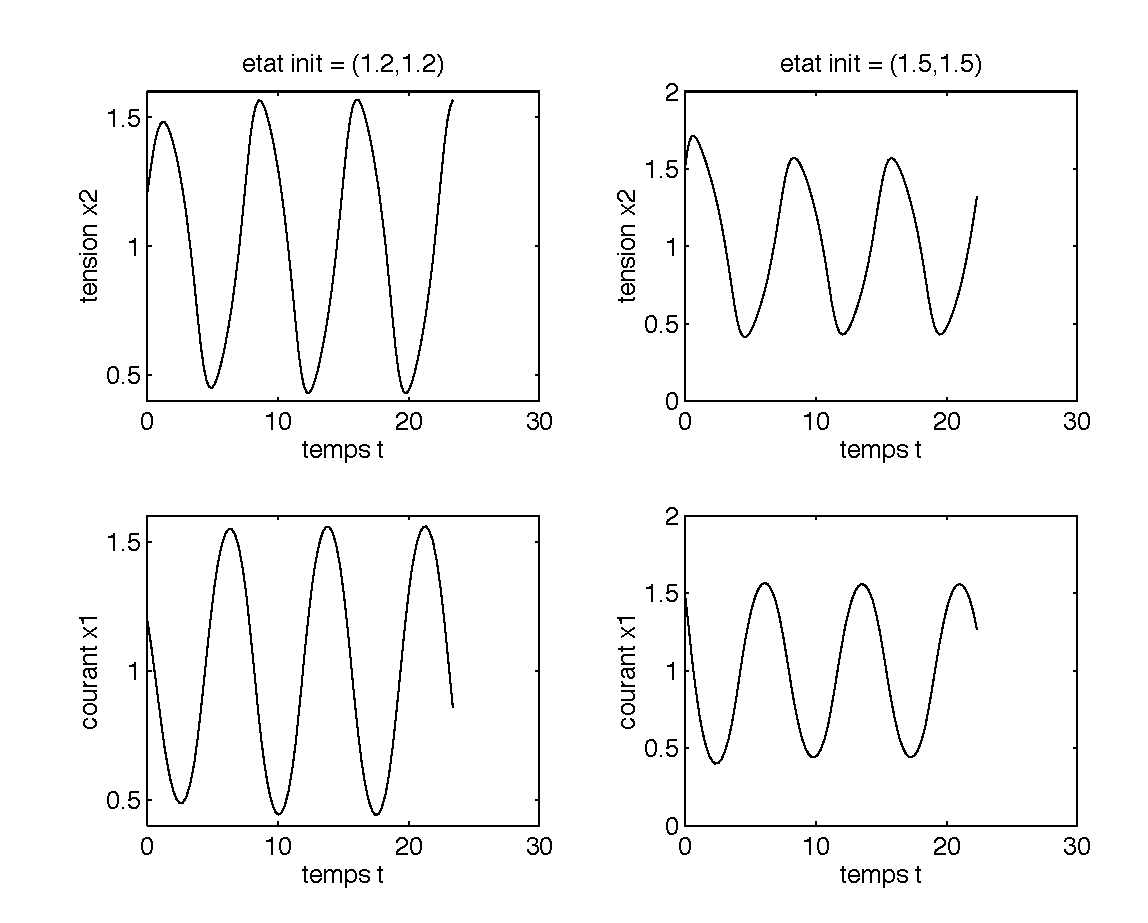
\includegraphics[width=10cm]{diodet} 
   \caption{Trajectoires du circuit {à} diode tunnel}
   \label{fig:simudiodet}
\end{figure}

Asymptotiquement, le syst{è}me conna\^{\i}tra  donc des oscillations   
d'amplitude  constante, quelle que soit la valeur des conditions initiales,
contrairement {à} ce qui se passe pour un syst{è}me lin{é}aire poss{é}dant
un {é}quilibre de type centre. En fait, c'est exactement ce que l'on cherche {à}
obtenir lorsque l'on construit un oscillateur : des oscillations d'amplitude
constante ind{é}pendamment des conditions initiales, qu'on ne peut donc obtenir
qu'avec un syst{è}me non lin{é}aire. Enfin, on peut aussi montrer que ce cycle limite est
structurellement stable, ce qui est {é}galement une propri{é}t{é} int{é}ressante pour la
conception d'un oscillateur. 
\qed
\end{exemple}

Nous formalisons ci-dessous quelques-unes des notions qui viennent d'{ê}tre d{é}crites dans l'exemple précédent.
Consid{é}rons un syst{è}me plan $$\dot x=f(x,\bar u)$$ avec entrée constante $\bar u$ et notons $x(t,x_0,\bar u)$ la solution au temps $t$ avec $x(0)=x_0$.

\begin{definition}{\bf\em Point limite}

Le point $z$ est un {\em point limite de $y$} pour le syst{è}me dynamique  
soumis {à} une
entr{é}e constante $\bar u$  s'il existe une suite $\{t_n\}$ dans
$\RR$ telle que $t_n \rightarrow \infty$ lorsque $n \rightarrow \infty$ et
$\lim_{n\rightarrow \infty} x(t_n,y,\bar u)=z$.\qed
\end{definition}

Conform{é}ment {à} cette d{é}finition, un {é}quilibre atttractif est donc un
point limite de tout point dans son bassin d'attraction. Mais la
notion de point limite est plus g{é}n{é}rale comme nous le
constaterons ci-dessous.

\begin{definition}{\bf \em Cycle limite}

{\em Un {\em cycle limite} est une orbite ferm{é}e $\gamma$ telle qu'un point de $\gamma$ est
un point limite d'un autre point du plan de phase n'appartenant pas
 {à} $\gamma$.}\cqfd\end{definition}
   
Cette d{é}finition montre que lorsqu'une orbite ferm{é}e est un cycle
limite, tout point de cette orbite est un point limite, et donc que la
trajectoire du syst{è}me s'approchera de plus en plus de chacun des
points de cette orbite ferm{é}e, {\em {à} des instants
  d{é}termin{é}s}.

Nous pouvons {é}noncer maintenant quelques r{é}sultats permettant d'{é}tablir l'existence
de trajectoires p{é}riodiques et de cycles limites. Ces r{é}sultats ne sont valables que
pour les syst{è}mes plans (alors qu'il existe également des cycles limites
pour des syst{è}mes d'ordre sup{é}rieur). La raison en est que les d{é}monstrations de ces
r{é}sultats reposent sur le fait qu'en dimension 2, une orbite ferm{é}e dans le plan de
phase divise ce plan en une r{é}gion int{é}rieure {à} l'orbite et une r{é}gion
ext{é}rieure, ce qui n'est bien s{\^u}r plus vrai dans un espace de phase de dimension
sup{é}rieure à 2.
Le premier r{é}sultat est une condition {\em suffisante} de {\em non-existence} de
trajectoire p{é}riodique (et donc de cycle limite).

\begin{theoreme} {\bf \em Bendixson Dulac, 1901 et 1933} 

{\em
Soit $D$ un domaine simplement connexe\footnote{un domaine simplement connexe dans  $\RR^2$ est un
domaine dont la fronti{è}re peut {ê}tre obtenue comme d{é}formation continue d'un cercle.}
dans $\RR^2$.  Si $${\mbox div}f \triangleq \frac{\partial f_1}{\partial
x_1}+\frac{\partial f_2}{\partial x_2}$$ est non identiquement nulle dans un sous-domaine
de $D$ et ne change pas de signe dans ce sous-domaine, alors $D$ ne contient pas d'orbite
ferm{é}e.}\cqfd\end{theoreme}

Rappelons que la divergence  ${\mbox div}f$ décrit l'éloignement (${\mbox div}f >0$) ou le rapprochement (${\mbox div}f <0$) issues de $\dot{x}=f(x)$.
Ce théorème se prouve simplement par contraposition: supposons qu'il existe une trajectoire fermée $\gamma$ dans le domaine, dont l'intérieur est $D_{\gamma} \subseteq D$. Alors 
l'intégrale de la divergence à l'intérieur de $\gamma$, $\int_{D_\gamma}  {\mbox div}f$ est égale par le théorème de Green-Stokes à l'intégrale de flux à travers la frontière $\gamma$ $\int_\gamma \langle f, n \rangle$, où $\langle.,.\rangle$ est le produit scalaire et $n$ est le vecteur normal unitaire sortant à $\gamma$. Cette dernière intégrale est nulle, puisque $f$ est tangent en tout point de la trajectoire $\gamma$. Il en résulte que la divergence ${\mbox div}f$ ne peut être partout négative ou partout positive dans $D_{\gamma}$.

Le deuxi{è}me r{é}sultat permet, lui, de mettre en {é}vidence l'existence d'un cycle
limite.  

\begin{theoreme} {\bf \em Poincar{é}-Bendixson, 1901}

Si $E$ est un sous ensemble fermé et borné de $\RR^2$, invariant  pour le système
$\dot x= f(x,\bar u)$, et si $\gamma$ est une orbite qui d{é}marre dans $E$, alors~:
\begin{itemize}
\item[i)] Si $E$ ne contient pas de point d'{é}quilibre, alors $\gamma$ est une orbite
p{é}riodique ou converge vers un cycle limite.
\item[ii)]Si $E$ ne contient pas d'orbite p{é}riodique mais contient un point d'{é}quilibre
unique, cet {é}quilibre est globalement attractif dans $E$. \qed
\end{itemize}
\end{theoreme}


Ce th{é}or{è}me peut {ê}tre utilis{é} effectivement pour d{é}montrer l'existence d'un
cycle limite. Pour ce faire, on cherche d'abord un ensemble ferm{é} born{é} et invariant.
Pour v{é}rifier que l'ensemble est bien invariant, on montre que sur la fronti{è}re de cet
ensemble, le champ de vecteurs pointe vers l'int{é}rieur. Ensuite, si on a pu exclure la
pr{é}sence d'{é}quilibres dans cet ensemble, celui-ci doit n{é}cessairement contenir un
cycle limite, ou ne contenir que des trajectoires p{é}riodiques.

Il est important de noter que ces deux théorèmes, contrairement à d'autres résultats de ce chapitre, sont spécifiques aux systèmes plans, et restreignent fortement les dynamiques possibles en deux dimensions: les trajectoires convergent vers un point, un cycle, ou sont non bornées. Les dimensions supérieures recèlent des comportements plus riches qui dépassent le cadre de ce cours: chaos, attracteurs étranges, etc.

\begin{exemple}{\bf \em Circuit {à} diode tunnel (suite)}

Nous reprenons le circuit d{é}j{à} d{é}crit avec les m{ê}mes valeurs
 num{é}riques que
pr{é}c{é}demment, qui conduisent {à} un {é}quilibre unique r{é}pulsif 
$(\bar x_1, \bar
x_2, \bar u)=(1,1,E-1)$, avec $E>1$. Prenons maintenant dans le plan de phase un cercle
centr{é} en
$(0,0)$ et de rayon suffisamment grand et montrons que, sur ce cercle, le champ de
vecteurs pointe vers l'int{é}rieur. Il s'agit donc de montrer que le produit scalaire du
champ de vecteurs et de la normale au cercle est n{é}gatif~: $PS=x_1f_1(x_1,x_2,\bar
u)+x_2f_2(x_1,x_2,\bar u)  < 0$. Choisissons comme rayon $r=\sqrt{2}\frac{E}{E-1}$ (voir
figure~\ref{bendiode}).
\begin{figure}[htbp] 
   \centering
   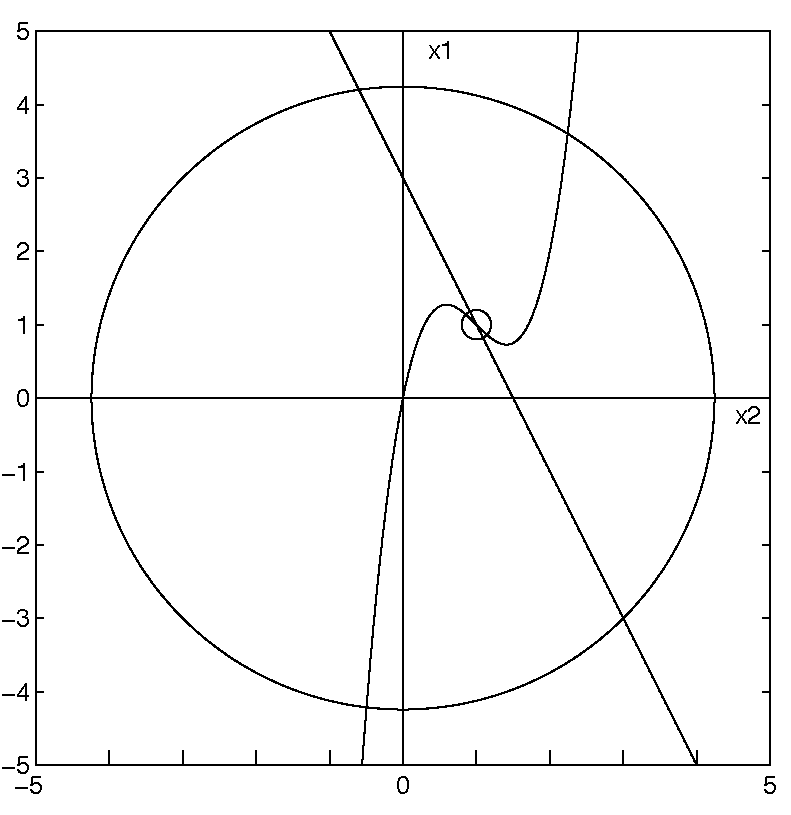
\includegraphics[width=10cm]{bendiode} 
   \caption{Ensemble invariant pour le circuit {à} diode tunnel}
   \label{bendiode}
\end{figure}
Le produit scalaire vaut $PS=-(E-1) x_1^2+E x_1-x_2h(x_2)$.
Remarquons que la quantit{é} $-x_2h(x_2)$ est toujours strictement n{é}gative sauf en $x_2=0$. Pour $x_1
\leq 0, PS < 0$. De m{ê}me, pour $x_1 \geq \frac{E}{E-1}, E x_1 \leq (E-1)x_1^2$ et $PS
<0$. Il reste
{à} {é}tudier la portion de cercle o{ù} $x_1 < \frac{E}{E-1}, x_2 > \frac{E}{E-1}.$ Un
petit calcul permet de v{é}rifier que $|h(x_2)| > |x_2|$ et que les in{é}galit{é}s
suivantes sont donc v{é}rifi{é}es ~:
\eqnn x_2h(x_2)&>x_2^2&>\frac{E^2}{(E-1)^2}\\
E x_1&<\frac{E^2}{E-1}&<\frac{E^2}{(E-1)^2}
\eeqnn
et donc $PS < 0$. Sur ce cercle de rayon $r$, le champ de vecteurs est donc rentrant. Par
ailleurs, comme l'{é}quilibre $(1,1,E-1)$ est r{é}pulsif, on peut prendre un cercle
suffisamment petit autour de cet {é}quilibre tel que le champ de vecteurs {é}valu{é} sur
ce cercle pointe vers l'ext{é}rieur.  Si l'on consid{è}re maintenant le domaine form{é} de
l'anneau  (non centr{é}) compris entre le petit cercle et le grand, il s'agit bien d'un
ensemble invariant puisque sur la fronti{è}re de cet ensemble, le champ de vecteurs pointe
vers l'int{é}rieur du domaine. Ce domaine ne comprenant aucun {é}quilibre, il doit donc
contenir un cycle limite (ou ne contenir que des trajectoires
p{é}riodiques). \qed
\end{exemple}



%Notons encore qu'il existe d'autres ensembles attractifs que des {é}quilibres %ou des
%cycles limites. Un syst{è}me comprenant trois {é}quilibres dont deux sont des %foyers
%instables et le troisi{è}me un col peut avoir un portrait de phase comme %illustr{é} {à} la
%figure~\ref{fig:syshuit}. Dans cet exemple, le ``huit'' illustr{é} sur la figure %est
%l'ensemble attractif pour tous les points {à} l'ext{é}rieur de cette courbe %ferm{é}e,
%alors que chacune de ses branches est l'ensemble attractif des points {à} %l'int{é}rieur.
%Les branches du ``huit'' sont des orbites de trajectoires tendant vers le col %(et ne sont
%donc pas des orbites p{é}riodiques).

%\begin{figure}
%\vspace*{6cm}
%\caption{ensemble attractif complexe}\label{fig:syshuit}
%\end{figure}

\section{Bifurcations}

Nous avons choisi d'{é}tudier dans ce chapitre l'allure des trajectoires de syst{è}mes plans pour une valeur constante de l'entr{é}e, $\bar u$. Cette valeur n'{é}tant pas
n{é}cessairement fix{é}e {\em a priori}, il est int{é}ressant d'analyser dans quelle
mesure les trajectoires seront influenc{é}es par des changements de $\bar u$. Le
th{é}or{è}me~\ref{Hart} nous donne d{é}j{à} une indication. Tant que l'{é}quilibre autour
duquel on analyse les trajectoires est hyperbolique, de petites variations de $\bar u$ ne
d{é}placeront pas beaucoup les valeurs propres de la matrice d'{é}tat de l'approximation
lin{é}aire du syst{è}me, et l'allure des trajectoires restera similaire. Mais en faisant
varier l'entr{é}e constante $\bar u$, il peut arriver que les
valeurs propres de la matrice d'{é}tat atteignent l'axe imaginaire du plan complexe, et
dans ce cas il faut s'attendre
{à} une modification fondamentale de l'allure des trajectoires. Plus globalement, les
diagrammes d'{é}quilibre {é}tudi{é}s au chapitre pr{é}c{é}dent montrent {é}galement qu'en
faisant varier $\bar u$, on peut modifier le nombre de points d'{é}quilibre du syst{è}me,
autant que leur nature. L'{é}tude des modifications de la nature et/ou du nombre des
{é}quilibres en fonction de l'{é}volution de l'entr{é}e du syst{è}me
rel{è}ve de ce qu'on appelle la th{é}orie des bifurcations, et l'entr{é}e constante $\bar u$ est alors
appel{é}e {\em param{è}tre de bifurcation}. Nous illustrons ci-dessous ce concept en
pr{é}sentant quatre types de bifurcations qui se rencontrent dans les syst{è}mes plans.

\subsection{Bifurcation de Hopf}

\begin{exemple} {\em\bf Circuit {à} diode tunnel (suite)}

Reprenons à nouveau l'exemple du circuit à diode tunnel en faisant varier l'entr{é}e 
$\bar u$ (c.{à}.d. la r{é}sistance variable $R$), avec une source de tension constante $E=1.5$.
La  figure~\ref{fig:eqdiohop} illustre comment l'{é}quilibre unique se d{é}place lorsque $\bar u$ varie. Le tableau suivant caract{é}rise le type d'{é}quilibre rencontr{é} en fonction de $\bar u$.
\begin{figure}[htbp] 
\centering
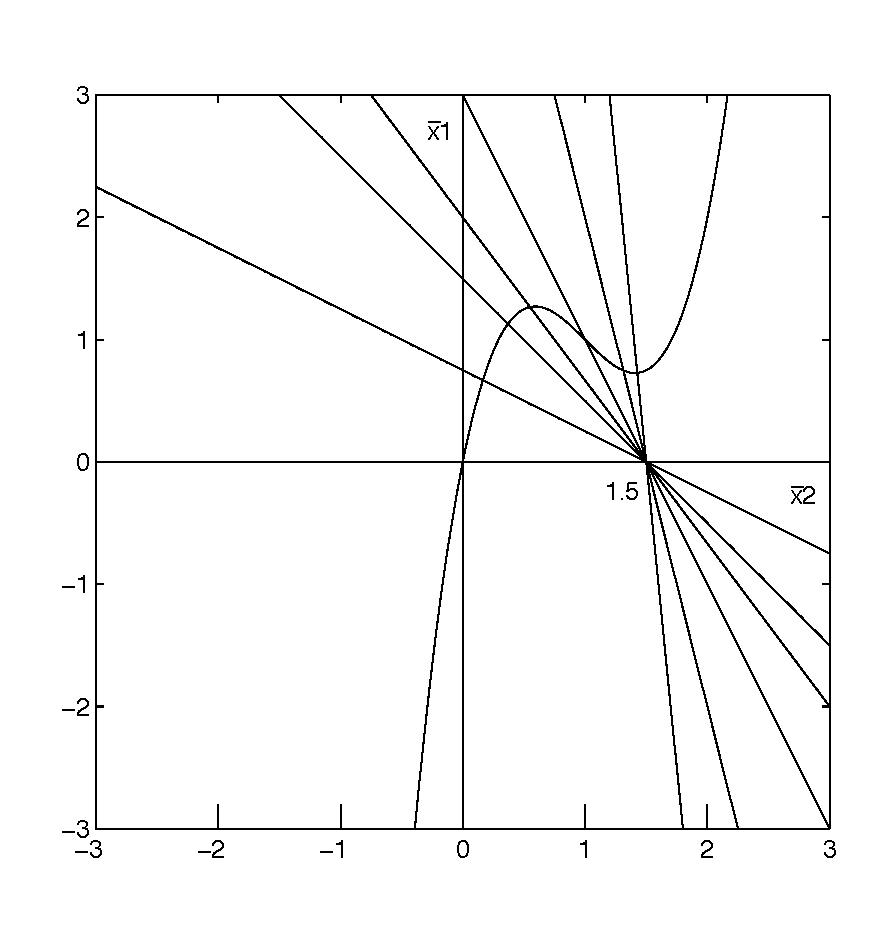
\includegraphics[height=65mm]{eqdiohop} 
\caption{Equilibre du circuit à diode tunnel lorsque la résistance $R$ varie.}
\label{fig:eqdiohop}
\end{figure}
\begin{table}
\begin{tabular}{|c|c|c|c|c|}\hline
$\bar u$&$\bar x_2$&$h'(\bar x_2)$&valeurs&type\\ 
&&&propres&d'{é}quilibre\\ \hline
$\bar u >0.7139$&$\bar x_2 < 0.5918$&$h'(\bar x_2)>0$&$\lambda_{1,2} \in C^-$&foyer\\
&&&&attractif\\ \hline
$0.1261<\bar u$&$0.5918< \bar x_2 $&$h'(\bar x_2)<0$&$\lambda_{1,2} \in  
C^+$&foyer\\ $<.7139$&$< 1.4082$&&&répulsif\\ \hline
$\bar u<0.1261$&$ \bar x_2 > 1.4082$&$2.5 >h'(\bar x_2)>0$&$\lambda_{1,2} \in
  C^-$&foyer\\
&&&&attractif\\ \hline
\end{tabular}
\end{table}
D{è}s lors, si l'on part d'une valeur de  la r{é}sistance variable $\bar u$ suffisamment grande, telle que le point d'{é}quilibre se
trouve {à} gauche du premier sommet de la courbe caract{é}ristique de la diode, et que
l'on diminue progressivement cette valeur, on passe successivement par les configurations suivantes~:  un foyer attractif, un foyer répulsif (associ{é} {à} un cycle limite), un foyer
attractif. Au moment des deux transitions entre foyer attractif et
répulsif, le syst{è}me passe par une valeur telle que le point d'{é}quilibre n'est pas
hyperbolique. 
\qed
\end{exemple}

La bifurcation que nous venons de mettre en {é}vidence
(passage d'un foyer attractif {à} un foyer répulsif accompagn{é} d'un cycle limite, ou l'inverse) est
appel{é}e {\em bifurcation de Hopf}. Le th{é}or{è}me suivant garantit d'ailleurs
l'existence d'un cycle limite. Afin de l'{é}noncer de fa\c con pr{é}cise, formalisons ce qui pr{é}c{è}de.  Soit un syst{è}me plan poss{é}dant une famille d'{é}quilibres uniques $(\bar x, \bar u)$ param{é}tr{é}e par $\bar u$. On suppose qu'il existe une valeur $\bar u^*$ de $\bar u$ 
telle que les valeurs propres de la matrice Jacobienne évaluée en cet
 {é}quilibre ont une partie r{é}elle nulle et une partie imaginaire non nulle. Ces valeurs propres d{é}pendent contin{\^u}ment de $\bar u$, au moins dans un voisinage de $\bar u^*$, et on les notera donc $$\lambda_i(\bar u)=\alpha(\bar u)\pm i \beta(\bar u).$$ On suppose en outre que $\frac{d\alpha(\bar u^*)}{d\bar u}>0$.

\begin{theoreme}
Avec les hypoth{è}ses qui pr{é}c{è}dent, si pour des valeurs de
 $\bar u$ proches de $\bar u^*$, l'{é}quilibre est attractif 
 pour $\bar u <\bar u^*$ et répulsif pour $\bar u >\bar u^*$ alors il
  existe une orbite ferm{é}e pour $\bar u>\bar u^*$ ou pour $\bar u<\bar u^*$. 
  En particulier, si $(\bar x^*,\bar u^*)$ est localement
   attractif, alors il existe un cycle limite attractif autour de 
  $(\bar x,\bar u)$ pout tout $\mu=\bar u-\bar u^*>0$, suffisamment petit.
   De plus, l'amplitude du cycle limite augmente lorsque $\mu$ augmente.
   \qed
\end{theoreme}
   
\begin{remarque}
Tel quel, l'{é}nonc{é} du th{é}or{è}me reste 
ambigu quant {à} la nature (attractive ou r{é}pulsive) de l'orbite 
ferm{é}e qui apparaît. On peut lever cette ambiguïté au prix 
d'un {é}nonc{é} plus technique faisant apparaître explicitement 
les termes d'ordre trois du syst{è}me non lin{é}aire
(voir par exemple Guckenheimer et Holmes, 
{\em Nonlinear Oscillations, Dynamical Systems, and Bifurcations of Vector 
Fields}, Springer-Verlag, 1983). 
\end{remarque}

\subsection{Bifurcation transcritique}

Consid{é}rons  la r{é}action $$X_1
+ X_2 \rightarrow 2 X_2$$ se produisant dans un r{é}acteur {à} volume constant, aliment{é}
en r{é}actif $X_1$ {à} la concentration $x_1^{in}$, avec un taux de dilution $u$.

Le mod{è}le d'état du syst{è}me (en supposant une cin{é}tique de r{é}action d{é}crite
par la loi d'action des masses) est donn{é} par
\eqnn
\dot x_1&=& -kx_1x_2+u(x_1^{in} -x_1)\\
\dot x_2&=& kx_1x_2-ux_2.
\eeqnn

Le syst{è}me poss{è}de deux {é}quilibres distincts pour chaque valeur constante de
l'entr{é}e $\bar u \neq kx_1^{in}$~: $(x_1^{in},0,\bar u)$ et $(\bar u/k,x_1^{in}-\bar
u/k,\bar u)$, comme illustr{é} {à} la figure~\ref{fig:diageqtc}.
\begin{figure}[htbp] 
   \centering
   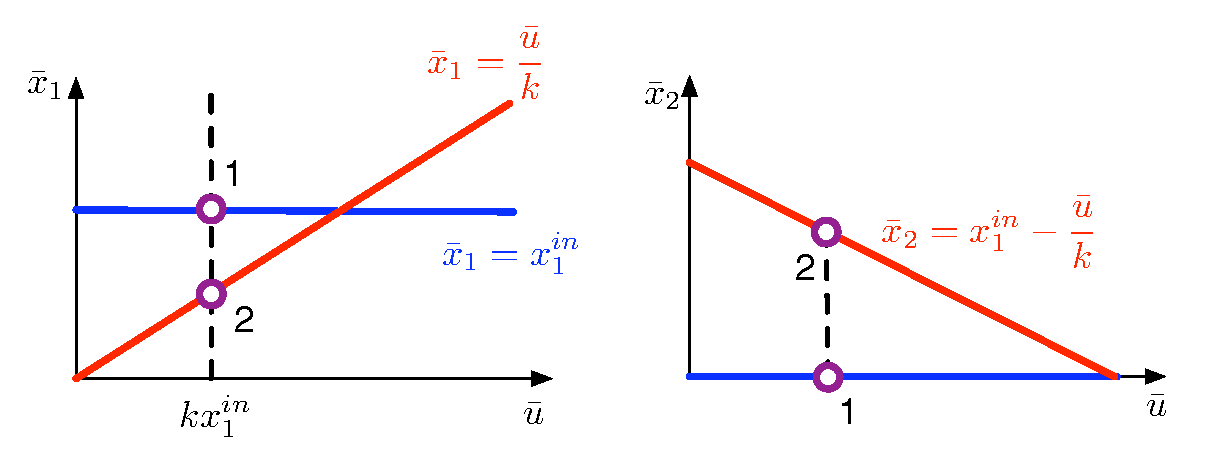
\includegraphics[height=4.6cm]{diageqtc} 
   \caption{Diagramme d'{é}quilibres - Bifurcation transcritique}
   \label{fig:diageqtc}
\end{figure}
On v{é}rifie facilement que le premier {é}quilibre est attractif si $\bar u > kx_1^{in}$ et
est un col sinon. Inversement, le deuxi{è}me {é}quilibre est attractif pour les petites
valeurs de $\bar u$ et devient un col si  $\bar u > kx_1^{in}$. Il y a donc ici aussi une
bifurcation, plus simple toutefois, les caract{é}ristiques des deux {é}quilibres {é}tant
{é}chang{é}es lorsque le param{è}tre de bifurcation $\bar u$ franchit la valeur critique
$kx_1^{in}$. Cette bifurcation est appel{é}e {\em bifurcation transcritique}. On
v{é}rifie {é}galement qu'{à} cette valeur critique, l'{é}quilibre (unique) est non
hyperbolique.

\subsection{Bifurcation col-noeud}

Le troisi{è}me type de bifurcation est illustr{é} par l'exemple du r{é}acteur chimique
exothermique d{é}crit {à} la section~7.1. Rappelons que le diagramme d'{é}quilibre
reliant la temp{é}rature d'{é}quilibre du r{é}acteur, $\bar T$, {à} l'apport calorifique
externe, $\bar u$, a l'allure illustr{é}e {à} la figure~\ref{fig:diageqcn}.
\begin{figure}[htbp] 
   \centering
   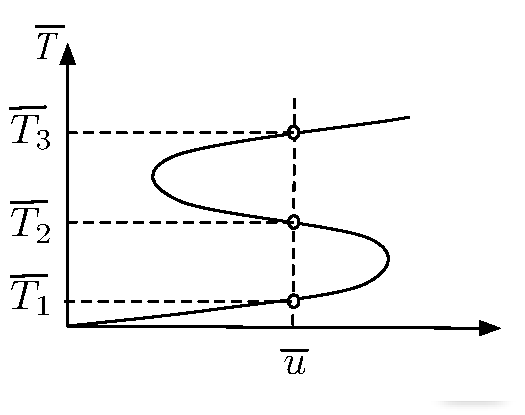
\includegraphics[height=5cm]{diageqcn} 
   \caption{Diagramme d'{é}quilibres - Bifurcation col-noeud}
   \label{fig:diageqcn}
\end{figure}
On constate donc que pour de faibles valeurs de $\bar u$, le syst{è}me poss{è}de un seul
point d'{é}quilibre correspondant {à} une temp{é}rature d'{é}quilibre basse et {à} une
grande concentration de r{é}actif dans le r{é}acteur (et d{è}s lors une faible
concentration du produit de la r{é}action). On peut v{é}rifier que cet {é}quilibre est
attractif. Puis, pour une valeur critique de $\bar u$ que l'on rep{è}re facilement sur le
diagramme d'{é}quilibre, le syst{è}me passe {à} trois valeurs d'{é}quilibre pour la
temp{é}rature, celle du milieu correspondant {à} un {é}quilibre attractif et les deux autres
{à} des {é}quilibres répulsifs. Enfin, en augmentant encore $\bar u$, on franchit une
nouvelle valeur critique au del{à} de laquelle le syst{è}me ne poss{è}de plus qu'un seul
{é}quilibre, attractif {é}galement. Il s'agit ici de {\em bifurcation col-noeud}. A partir
d'une valeur critique de l'entr{é}e (c.{à}.d. du param{è}tre de bifurcation) apparaissent
deux nouveaux {é}quilibres, l'un d'eux {é}tant un noeud attractif, l'autre {é}tant un col.
A la valeur critique, l'{é}quilibre n'est pas hyperbolique.

\subsection{Bifurcation fourche}

Le mécanisme illustré à la figure \ref{fig:regwatt} est un \og régulateur de Watt \fg.  Ce dispositif peut servir à mesurer une
vitesse de rotation à partir d'un pointeur fixé sur l'axe vertical, ou, et
c'est pour cela qu'il a été inventé, à réguler cette vitesse si le pointeur
est relié à une vanne d'alimentation du moteur faisant tourner
le dispositif.
\begin{figure}[htbp] 
   \centering
   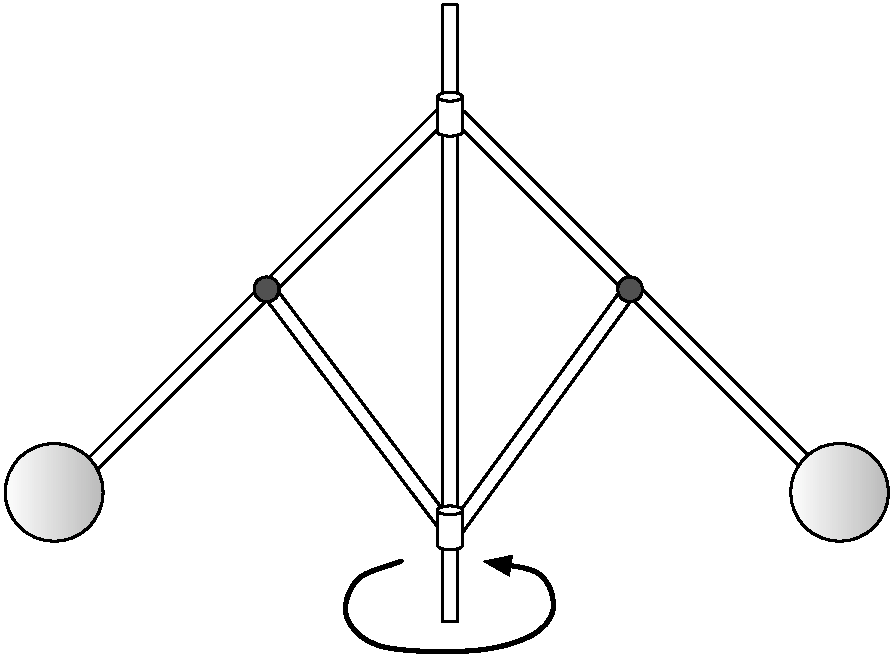
\includegraphics[height=4cm]{regwatt} \hspace{2cm}
   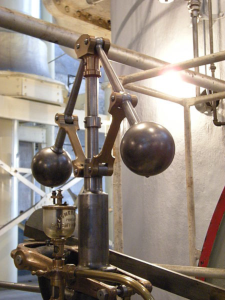
\includegraphics[height=4cm]{photo-regwatt} 
   \caption{Régulateur de Watt}
   \label{fig:regwatt}
\end{figure}
On peut vérifier que les équations décrivant le mouvement du système s'écrivent :
\eqnn
\dot x_1 &=& x_2\\
\dot x_2 &=& u^2\cos x_1 \sin x_1 -k \sin x_1 -Kx_2
\eeqnn
où $x_1 = \theta$ est la position angulaire des pendules symétriques et $u$ est la vitesse de rotation.

Ce dispositif a un équilibre en $(x_1, x_2, u)=(0,0, \bar u)$ et, si $\bar
u^2 > k,$ un autre équilibre en $(\bar x_1 = \mbox{ arc }\cos \frac{k}{\bar u^2}, 0,
\bar u)$ avec $\bar x_1 \in [0,\frac{\pi}{2}]$.  En fait $(-\bar x_1, 0, \bar
u)$ est aussi un équilibre qui correspondrait à la permutation des deux
pendules, ce qui est (physiquement) impossible mais conceptuellement
possible, d'après les équations ci-dessus.

La matrice Jacobienne du système autour de l'équilibre $(0,0, \bar u)$
s'écrit :
$$
A = \bma{cc}0 & 1\\ \bar u^2-k & -K
\ema
$$
Cet équilibre est attractif pour $\bar u^2 < k$ et répulsif pour $\bar u^2>k$.  Pour $\bar u^2
= k$, l'équilibre n'est pas hyperbolique.

Autour des deux autres équilibres, la matrice Jacobienne devient :
$$
A = \bma{cc} 0 & 1\\ \frac{k^2}{\bar u^2} -\bar u^2 & -K \ema \mbox{ avec } \bar u^2 > k
\Rightarrow \bar u^4 > k^2
$$
Ces équilibres sont donc attractifs.  Le diagramme de bifurcation peut alors
s'illustrer comme indiqué à la figure \ref{fig:biffourche}.  Il s'agit d'une bifurcation de
type fourche.
\begin{figure}[htbp] 
   \centering
   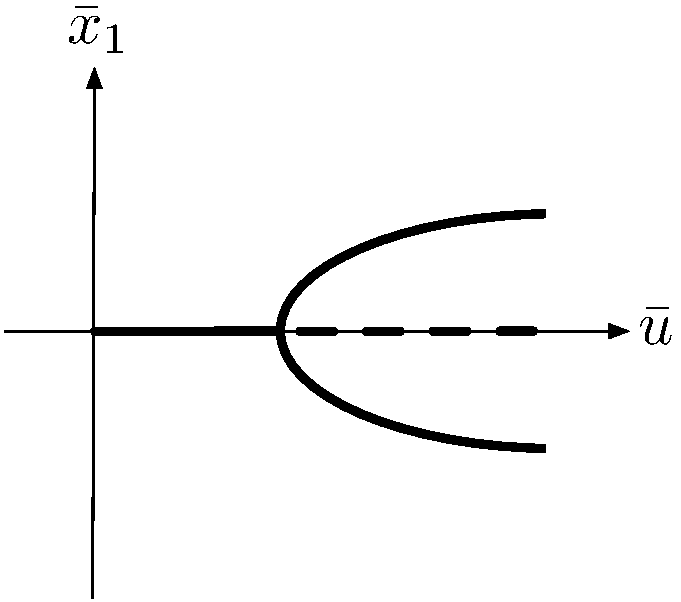
\includegraphics[height=5cm]{biffourche} 
   \caption{Diagramme d'équilibres - bifurcation fourche}
   \label{fig:biffourche}
\end{figure}
 
\subsection{Généralisations}

Nous avons d{é}crit dans cette section les bifurcations
relatives {à} des syst{è}mes d'ordre deux d{é}pendant d'un param{è}tre (la valeur de $\bar
u$). Ces bifurcations sont caract{é}ris{é}es par la travers{é}e de l'axe imaginaire du
plan complexe par une valeur propre r{é}elle de l'approximation lin{é}aire ou par une
paire de valeurs propres complexes conjugu{é}es (bifurcation de Hopf).  Lorsqu'un
syst{è}me d'ordre plus grand que deux d{é}pend d'un param{è}tre variable, il est rare que
plus d'une valeur propre r{é}elle (ou plus d'une paire de valeurs propres complexes
conjugu{é}es) franchisse l'axe imaginaire pour la m{ê}me valeur du param{è}tre de
bifurcation. Ce que nous venons de d{é}crire s'observe d{è}s lors aussi, dans des espaces
de phase plus compliqu{é}s {à} visualiser, pour des syst{è}mes d'ordre
 sup{é}rieur.  

\newpage
\section{Exercices}
\markboth{{\bf \hspace*{5mm} Chapitre 8}\hfill
Systèmes plans}
{{\bf Sec. \thesection}\hfill Exercices
\hspace*{5mm}}
 
\begin{exercice} {\bf \em Un système mécanique}

On considère un robot manipulateur à un segment relié à un
chassis  fixe par une articulation rotoïde. Le robot se déplace dans un
plan vertical. Il est actionné par un moteur produisant un couple
appliqué
à l'articulation et est soumis à un couple de frottement visqueux. La
flexibilité est négligée.
\begin{enumerate}
\item Etablir le modèle d'état du système.
\item Déterminer les configurations d'équilibre.
\item Analyser le comportement des trajectoires au voisinage des
équilibres en cas de frottement visqueux linéaire quand le couple
appliqué est constant.
\item Que peut-on dire des équilibres quand le frottement visqueux
est quadratique ?
\end{enumerate}
\end{exercice}
\vv

\begin{exercice}{\bf \em Un réacteur chimique}

Soit un réacteur continu parfaitement mélangé et à volume
constant dans lequel se déroule une réaction chimique 
irréversible mettant en oeuvre deux espèces $A$ et $B$~:
\eqnn
A \longrightarrow B.
\eeqnn
Le réacteur est alimenté uniquement avec l'espèce $A$, à
débit volumique constant strictement positif. La variable d'entrée est
la concentration d'alimentation du réacteur. La cinétique de réaction
est une fonction des concentrations des deux espèces : $r(x_A,x_B)$. 
\begin{enumerate}
\item Etablir le modèle d'état du système.
\item Montrer que, à entrée constante,  l'équilibre est unique et
stable si la cinétique obéit à la loi d'action des masses avec inhibition
hyperbolique par le produit.  Est-ce un noeud ou un foyer ?
\item Montrer que le système peut avoir des équilibres instables 
si la cinétique est une fonction monotone croissante de ses
arguments. 
\end{enumerate}
\end{exercice}
\vv

\begin{exercice} {\bf \em Un système à compartiments}

Quelles sont les conditions sur la structure du graphe d'un
système linéaire à deux compartiments pour que le système ait
une ou deux valeur propres nulles ? Quel est alors le comportement du
système (détailler les différents cas possibles) ?
\end{exercice}
\vv

\begin{exercice}{\bf \em Génératrice DC avec auto-excitation}

On considère une génératrice DC avec auto-excitation. La tension induite est, à vitesse constante, une fonction {\em monotone
croissante bornée} du courant d'excitation $E(I_s)$ telle que $E(0) >
0$. La génératrice débite sur une charge résistive. L'entrée de
commande du système est la vitesse de rotation de la
génératrice.
\begin{enumerate}
\item Déterminer le modèle d'état du système.
\item Montrer qu'on peut choisir le sens de référence des courants pour que le système soit positif.
\item Quelle allure doit avoir la fonction $E(I_s)$ pour qu'il y ait trois
équilibres hyperboliques isolés à vitesse de rotation constante. Discuter la
stabilité de ces équilibres.
\item Etudier les bifurcations de la configuration d'équilibre en fonction de la vitesse de rotation.
\end{enumerate}
\end{exercice}
\vv

\begin{exercice} {\bf \em Circuit électrique RLC} 

On considère le circuit électrique linéaire suivant :
\begin{figure}[h] 
   \centering
   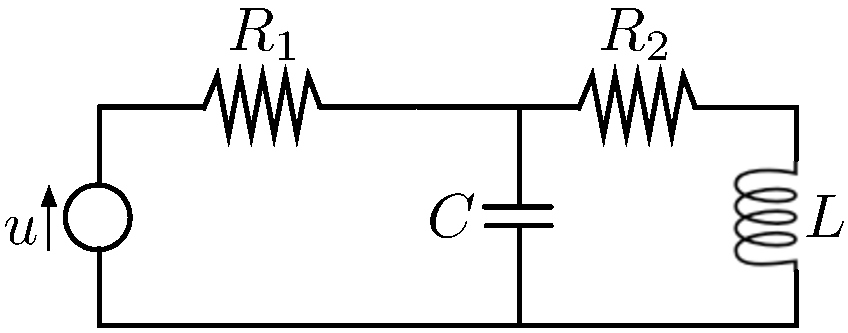
\includegraphics[height=25mm]{E8-5} 
   \caption{Circuit électrique RLC}
   \label{fig:E8-5}
\end{figure}

où $R_2 = 1\Omega, C = 1F$ et $L = 1H$.

\begin{enumerate}
\item Ecrire un modèle d'état.
\item Déterminer les équilibres.
\item Quelles sont les conditions sur $R_1$ pour que chaque équilibre soit un
noeud, un foyer ou un col?
\end{enumerate}

On considère le même circuit électrique mais avec $R_1 = 1\Omega$ et $R_2$ une résistance non
linéaire décrite par la relation tension-courant $v_r = i^3_r - 3i^2_r + i_r$
\begin{enumerate}
\item Calculer les équilibres du système.
\item Caractériser le comportement du système au voisinage de ces équilibres.
\end{enumerate}
\end{exercice}
\vv 

\begin{exercice}{\bf \em Modélisation d'une activité de pêche.}

Dans un lac vit une espèce de poissons dont la croissance obéit à une loi logistique. Les poissons sont capturés par des pêcheurs suivant un principe d'action des masses. Les pêcheurs sont attirés vers le lac avec un taux directement proportionnel à la quantité de poissons dans le lac. Par contre les  pêcheurs sont découragés de pêcher avec un taux directement proportionnel au nombre de pêcheurs déjà présents.
\begin{enumerate}
\item Etablir un modèle d'état du système.
\item Etudier l'existence et la stabilité des états d'équilibre.
\end{enumerate}
\end{exercice}


\end{document}